% !TeX document-id = {ca28df42-0773-4265-bb7c-b21d86ed4d82}
%%%%%%%%%%%%%%%%%%%%%%%%%%%%%%%%%%%%%%%%%%%%%%%%%
%
%	MSc THESIS TEMPLATE
%	developed for my master thesis at the Universitá di Torino
%
%	by Eugenio Senes (eugenio.senes@gmail.com)
%
%	released under MIT license, so share, modify and enjoy, but quoting the author !
%
%%%%%%%%%%%%%%%%%%%%%%%%%%%%%%%%%%%%%%%%%%%%%%%%%

%% DOCUMENT CLASS (alternative to book is 'report')
% Print just right page or both sides (comment the other one)
\documentclass[12pt,a4paper,openright,oneside]{book}	%%One sided
%\documentclass[12pt,a4paper,openright,twoside]{book}	%%Double sided

%% SET MARGINS OF THE PAGES
\usepackage{geometry}
\geometry{a4paper,portrait, left=35mm, right=20mm, top=35mm, bottom=30mm}

%% HEADERS AND FOOTERS
\usepackage{fancyhdr}
\pagestyle{fancy}
\fancyhf{} 			%clears default header and footer
\rhead{} 			%right head
\lhead{ \leftmark} 	%left head
\rfoot{\thepage}
%%consider using also chead, cfoot, lfoot
%coherce the plain stile to this (e.g. the first page of every chapter)
\fancypagestyle{plain}{
	\fancyhf{}
	\rfoot{\thepage}
	\renewcommand{\headrulewidth}{0pt}
	\renewcommand{\footrulewidth}{0pt}
}
%% CLEAR PAGE WITHOUT NUMBER AT THE BEGINNING OF CHAPTERS
\let\origdoublepage\cleardoublepage
\newcommand{\clearemptydoublepage}{%
  \clearpage
  {\pagestyle{empty}\origdoublepage}%
}
%% ALLOW PAGE ROTATION
\usepackage{lscape}
\usepackage[english, italian]{babel} %%Set Italian as main language of the document
%% HYPERTEXT SETUP
\usepackage{hyperref}
\usepackage{ragged2e}
\usepackage{enumerate}

%% redefinition of /autoref naming conventions to italian names
\addto\extrasitalian{
	\def\figureautorefname{Figura}
	\def\equationautorefname{Equazione}
	\def\subsectionautorefname{Sezione}
}
\hypersetup{
    colorlinks,
    citecolor=black,
    filecolor=black,
    linkcolor=black,
    urlcolor=black
}
%% PDF SETTINGS
\hypersetup{
    pdfauthor={Andrea Zito and Emanuele Rovaretto and Lorenzo Bafunno},
    pdftitle={shortTitle},
    pdfsubject={subject},
    pdfkeywords={Semantic Web, Type Systems, Haskell, OCaml}
}
%% FONTS AND SYMBOLS
\usepackage[utf8]{inputenc}	%%input font setting
\usepackage[T1]{fontenc} 		%%font for automatic recognition of letters with the accent
\usepackage{amsfonts}		%%fonts for the mathematical rendering of formulas
\usepackage{amssymb}
\usepackage{amsmath}
\usepackage{amsthm}
\usepackage{thmtools}
\newtheorem{theorem}{Theorem}
\usepackage{syntax}

\newtheorem{definition}{Definizione}
%% CHAPTERS STRUCTURE

%% FIGURES
\usepackage{graphicx}
\usepackage{subfigure}		%%allow side by side figures with single caption
%% TABLES
\usepackage{multirow}		%%allow to merge rows in the tables
\usepackage{booktabs}		%%allow use of \toprule, \midrule, \bottomrule in tables
%%CAPTIONS
\usepackage{caption}
%% BIBLIOGRAPHY
\usepackage[babel]{csquotes}
%% CODE LISTINGS
\usepackage{listings}		%%allow to use code listings

\usepackage{tikz}
\usepackage{prooftree}
\usepackage{minted}
\usemintedstyle{perldoc}
\usetikzlibrary{positioning,
                quotes}

%% HYPENATON
\hyphenation{te-si pip-po paperino}	%manual hyphenation
\definecolor{codegray}{gray}{0.9}
\newcommand{\singlenodegraph}[1]{
  \tikz{\node [rounded corners, scale=0.9, draw, fill=gray!30, font=\footnotesize] {#1}}
}
%%%%%%%%%%%%%%%%%%%%%%%%%%%%%%%%%%%%%%%%%%%%%%%%%
%%%% BEGIN DOCUMENT
\begin{document}

%%%%%% HEAD  OF THE DOCUMENT
\frontmatter
%%FRONT PAGE
%\begin{titlepage}
    %upper part

    %logo
    \begin{center}
        
\includegraphics[scale=.3]{head/logo.png}
    \end{center}
    %title
    \begin{center}
        \vspace{20mm}
        {{\Large{\textsc{\bf Universit\`a degli Studi di Torino \\} \vspace{2mm} \emph{Corso di Laurea in Informatica}}}}
        \vspace{5mm}
    \end{center}
    \begin{center}
        \vspace{5mm}
        {\LARGE{\bf THE FANCY TITLE\\ OF MY FANCY THESIS\\}}
        \vspace{3mm}
        {\large{Tesi di Laurea\\}}
        %\vspace{5mm}
        %{\LARGE{\bf SECOND ROW TITLE}}
    \end{center}
    \vspace{20mm}
    %relatore
    \par
    \noindent
    \begin{minipage}[t]{0.47\textwidth}
        {\large{\bf Relatore/Relatrice:\\}}
        {\large{
                Bono Viviana
            }}
        \vspace{8mm}
        {\large{\bf \\ Controrelatore:\\
                Prof.\\
                Zio Paperone}}
    \end{minipage}
    \\
    \null\hfill
    \begin{minipage}[t]{0.40\textwidth}
        \vspace{20mm}
        {\large{\bf Candidato:\\
                Lorenzo Bafunno\\
            } \large{Matricola 944233}}
    \end{minipage}
    \vspace{10mm}
    \begin{center}
        {\large{Anno Accademico 2022/2023}}
    \end{center}

\end{titlepage}
\begin{titlepage}
    %upper part

    %logo
    \begin{center}
        
\includegraphics[scale=.3]{head/logo.png}
    \end{center}
    %title
    \begin{center}
        \vspace{20mm}
        {{\Large{\textsc{\bf Universit\`a degli Studi di Torino \\} \vspace{2mm} \emph{Corso di Laurea in Informatica}}}}
        \vspace{5mm}
    \end{center}
    \begin{center}
        \vspace{5mm}
        {\LARGE{\bf THE FANCY TITLE\\ OF MY FANCY THESIS\\}}
        \vspace{3mm}
        {\large{Tesi di Laurea\\}}
        %\vspace{5mm}
        %{\LARGE{\bf SECOND ROW TITLE}}
    \end{center}
    \vspace{20mm}
    %relatore
    \par
    \noindent
    \begin{minipage}[t]{0.47\textwidth}
        {\large{\bf Relatore:}\\
            Bono Viviana}\\
        \vspace{4mm}
        \\
        {\large{\bf Correlatore:}\\
        Lieto Antonio\\
        Marco
        }
        %\vspace{8mm}
        %{\large{\bf \\ Controrelatore:\\
        %Prof.ssa Nonna Papera}}
    \end{minipage}
    \\
    \null\hfill
    \begin{minipage}[t]{0.40\textwidth}
        \vspace{20mm}
        {\large{\bf Candidato:\\
                Lorenzo Bafunno\\
            } \large{Matricola 944233}}
    \end{minipage}
    \vspace{10mm}
    \begin{center}
        {\large{Anno Accademico 2022/2023}}
    \end{center}

\end{titlepage}
\clearemptydoublepage
%%DEDICATION (the initial quote) & statement of originality
\thispagestyle{empty}
\begin{flushright}

    \vspace*{60mm}

    The amazing quote\\
    that I chose as inspiration\\
    for this work\\
    \vspace{4mm}
    Author, \textit{Title}\\




\end{flushright}

\vspace*{110mm}
\noindent
\emph{Dichiaro di essere responsabile del contenuto dell'elaborato che presento al fine del
    conseguimento del titolo, di non avere plagiato in tutto o in parte il lavoro prodotto da
    altri e di aver citato le fonti originali in modo congruente alle normative vigenti in
    materia di plagio e di diritto d'autore. Sono inoltre consapevole che nel caso la mia
    dichiarazione risultasse mendace, potrei incorrere nelle sanzioni previste dalla legge e
    la mia ammissione alla prova finale potrebbe essere negata.}
\clearemptydoublepage
%%ABSTRACT
\chapter{Abstract}
I linguaggi funzionali tipati, grazie a concetti come le funzioni di ordine superiore, i data type e il pattern matching, permettono di programmare in modo naturale applicazioni modulari e di facile debugging.  Questa loro flessibilità e le garanzie di correttezza che offrono (grazie al controllo statico dei tipi) pare adatta per la costruzione di formalismi e strumenti per supportare un reasoning efficiente nell'ambito della Knowledge representation. Si pone sempre più, infatti, il problema di avere efficienza e, nel contempo, offrire semantiche espressive, per i dati in formato Resource Description Framework (RDF). Il formato RDF è lo strumento base proposto da W3C per la codifica, lo scambio e il riutilizzo di metadati strutturati (tramite grafi detti Knowledge graph) e consente l'interoperabilità semantica tra applicazioni che condividono le informazioni sul Web. Questo lavoro è uno studio esplorativo sullo stato dell'arte e sui possibili sviluppi futuri dell'applicazione dei linguaggi funzionali tipati nel contesto della Knowledge representation, in generale, e dei dati in formato RDF, in particolare.
\clearemptydoublepage
%%INDEXES
%summary
\setlength{\headheight}{14.49998pt}
\tableofcontents
\clearemptydoublepage

%%%%%% BODY OF THE DOCUMENT
\mainmatter
\clearemptydoublepage
\chapter{Introduzione}
%\chapter{Introduzione}

\section{Scopo della ricerca}
\paragraph{} Questo lavoro è un lavoro di gruppo svolto in collaborazione con Lorenzo Bafunno e Andrea Zito e la consulenza del dottor Marco Antonio Stranisci, della professoressa Rossana Damiano e del professor Antonio Lieto.

L'idea di partenza è stata quella di studiare i benefici dell'applicazione dei linguaggi funzionali e dei sistemi di tipi statici
 rappresentazione della conoscenza. 
 
% ontologie
Le \emph{ontologie} rappresentano un formalismo molto diffuso per la rappresentazione della conoscenza. Un'ontologia si compone di due parti: \emph{T-Box} ( Terminology Box) e \emph{A-Box} (Assertion Box). La prima contiene formule logiche per modellare il dominio, per esempio per affermare che uno 'Studente' è una 'Persona'. La seconda è usata per esprimere asserzioni su individui, per esempio affermare che 'Emanuele' è un istanza di 'Persona'. Un ragionamento su un'ontologia è inferenza di proprietà di interesse, per esempio se si inferisce che 'Persona' ha un nome, allora anche 'Studente' ha un nome, in quanto sua sottoclasse. Le basi di conoscenza rappresentate da ontologie vengono interrogate tramite \emph{query}. Si dice che una query è \emph{abitata} (\emph{inhabited}) se  restituisce dei risultati. Per esempio, una query che cerca le istanze di una 'Pizza Margherita' che allo stesso tempo sia anche un 'Gelato', non è abitata perché potrà mai avere dei risultati, perché nessuna pizza è un gelato (almeno in una base di conoscenza basata sul senso comune).  Una trattazione più avanzata sul tema sarà presentata nel Capitolo \ref{chap:preliminaries}.

% motivazione e obbiettivo
\paragraph{} Dalla nostra indagine (si veda per esempio \cite{baader2017introductionDL}), è emerso che le ontologie non sono più utilizzate nella loro interezza (T-Box e A-Box) perché è troppo dispendioso eseguire ragionamenti formali complessi, anche se così facendo si perde espressività, ignorando una strutturazione più sofisticata dei concetti. Oggigiorno infatti si tende a utilizzare solamente gli A-Box, ovvero le asserzioni sugli individui, per esempio come dati per i modelli basati sul machine learning. Ci siamo quindi chiesti se fosse possibile costruire formalismi che recuperino parte dell'espressività dei ragionamenti formali, senza perdere troppo in efficienza. Una strada che riteniamo promettente è l'uso dei linguaggi funzionali e dei sistemi di tipo per creare applicazioni e nuovi linguaggi che manipolano ontologie spostando i controlli, che di norma vengono compiuti a run-time, a compile-time tramite i sistemi di tipaggio statico.     

\section{Il nostro lavoro}
\paragraph{} Abbiamo cominciato ad analizzare alcuni lavori appartenenti alla letteratura sulla rappresentazione della conoscenza, in particolare sulle ontologie. Abbiamo poi analizzato in dettaglio la tesi di dottorato di Martin Gerhard Leinberger \cite{leinbergerphdthesis}, il quale ha ideato un calcolo con sistema di tipi statico per verificare l'abitabilità delle query SPARQL-CQ trattato nel capitolo \ref{chap:preliminaries}. Noi abbiamo deciso di implementarlo. Bafunno e Zito hanno sottolineato la possibilità di usare un Reasoner (ovvero un sistema in grado di eseguire ragionamenti e deduzioni sulle basi di conoscena) già esistente, indicando HermiT come il più adatto. Per quanto riguarda il linguaggio da utilizzare, assieme a Zito, la prima idea è stata utilizzare Haskell, un linguaggio funzionale che già conoscevamo, ma alla fine la scelta è ricaduta su OCaml (che abbiamo studiato appositamente), un altro linguaggio funzionale più maturo, con più librerie e più interfacciabile con il modulo Reasoner rispetto ad Haskell. 

\paragraph{} Prese queste decisioni architetturali, ho cominciato lo studio per conoscere meglio le due risorse che avrei poi usato nell'implementazione: Hermit \cite{HermiT} e OCaml \footnote{www.ocaml.org}.\\
Ho studiato come utilizzare il reasoner HermiT, compito reso più arduo a causa della poca documentazione presente in rete. Per quanto riguarda OCaml, avendo già un background di Haskell, capire come utilizzarlo non è stato particolarmente impegnativo. \\

\paragraph{} Per l'implementazione, ho deciso di creare due moduli, il modulo Reasoner, scritto in Java, e il modulo OCaml, il primo che performa ragionamenti sull'ontologia, mentre il secondo che implementa il sistema di tipi di Leinberger.

Il mio primo problema è stato far dialogare i due moduli. La soluzione che ho trovato prevede che il modulo OCaml richiami la shell di comando, al quale viene delegata la responsabilità di lanciare il modulo Reasoner.

Un altro grosso problema è stato scegliere la "lingua veicolare" da utilizzare per far comunicare i due moduli: la prima idea è stata quella di definire una grammatica da zero, con tanto di parsificatore da dover usare nel Reasoner: una scelta troppo costosa. Allora ho provato a cercare qualche grammatica già esistente: ho trovato una sintassi sviluppata dall'Università di Manchester per la rappresentazione di ontologie OWL, un particolare tipo di ontologie, con un parsificatore già implementato \footnote{https://ceur-ws.org/Vol-216/submission_9.pdf}. Non rimaneva dunque che adattare il modulo OCaml a quella sintassi e integrare il parsificatore nel modulo Reasoner, per terminare il ponte fra i moduli.

\paragraph{} Il parsificatore e il lexer delle query nel modulo OCaml sono stati facili da realizzare, perché ho usato un generatore di parser e un generatore di lexer per OCaml, OCamlyacc e OCamllex, nei quale mi è bastato specificare la grammatica della query (illustrata nel dettaglio al Capitolo \ref{chap:preliminaries}) e la semantica dei token per ottenere il parsificatore e il lexer. L'unico intoppo l'ho registrato quando ho dovuto cercare di disambiguare la grammatica inizialmente implementata. 

\paragraph{} Il resto dell'implementazione è stato quasi immediato senza grossi problemi, dovendo solo implementare ciò che era già stato progettato da Leinberger.

Attorno al lavoro sull'implementazione del modulo delle query di Leinberger, riassunto sopra nella tesi si trovano:
\begin{itemize}
\item il lavoro di rassegna della letteratura sui tipi e Web Semantico, di cui si è occupato essenzialmente Lorenzo Bafunno (Capitolo \ref{chap:State-of-art});
\item l'implementazione del resto del calcolo di Leinberger, creata principalmente da Andrea Zito (Capitolo \ref{chap:Implementazione});
\item le direzioni di ricerca future, che nascono da riflessioni corali, supportate dal dottor Marco Antonio Stranisci, dalla professoressa Rossana Damiano e dal professor Antonio Lieto (Capitolo \ref{chap:FutureWork}).
\end{itemize}
%\textsl{Questo lavoro è stato fatto in collaborazione con Emanuele Rovaretto e Andrea Zito, sotto la supervisione della professoressa Viviana Bono e con la consulenza del dottor Marco Antonio Stranisci, della professoressa Rossana Damiano e del professor Antonio Lieto.}\\\\
\section{Semantic Web}
Il Web Semantico fornisce un framework comune che consente la condivisione e il riutilizzo dei dati al di là dei confini delle applicazioni.
 È uno sforzo collaborativo guidato dall'organizzazione W3C\footnote{\url{https://www.w3.org/about/}} con la partecipazione di un gran numero di ricercatori 
 e partner industriali. Gli obiettivi principali del Web Semantico \cite{berners2001semantic, hitzler2021review} sono due:
\begin{enumerate}[I)]
	\item creare una rete di dati interconnessi, in contrapposizione all'attuale Web basato sui documenti;
	\item permettere che una macchina possa comprendere le informazioni disponibili sul Web senza intervento umano.
\end{enumerate}
Per soddisfare entrambi, si è resa necessaria l'introduzione di annotazioni espressive che spieghino la correlazione fra i dati, ed è per questo che W3C ha 
introdotto il \textit{Resource Description Framework} (RDF) \cite{RDFspecification}. RDF è uno standard che permette la codifica, lo scambio e il riutilizzo 
di metadati (dati che descrivono altri dati), strutturandoli come dichiarazioni di triple soggetto, predicato e oggetto. In questo modo RDF permette di 
rappresentare dei grafi, i cui nodi e vertici rappresentano informazioni presenti nel web (chiamate \textit{risorse}) e sono identificate dagli IRI, 
identificatori unici di risorse che svolgono la stessa funzione degli URL per i documenti web. Essendo unici, essi consentono di associare ai nodi di due 
grafi diversi la stessa risorsa. Per condividere la terminologia (e.g. cosa s'intende per "Studente") è stato proposto da W3C un ulteriore standard, le 
ontologie OWL. In generale, le ontologie sono rappresentazioni formali, condivise ed esplicite di una concettualizzazione di un dominio di interesse 
\cite{goy2015ontologies} in maniera complessa e strutturata. OWL (\textit{Ontology Web Language}) è un linguaggio altamente espressivo e formale basato su 
logiche appartenenti al campo della knowledge representation (KR), le logiche descrittive (DL) \cite{baader2017introductionDL}. La forma logica delle 
ontologie OWL di definire un ragionamento automatico basato su inferenze, cioè dedurre nuove informazioni basandosi su quelle che sappiamo essere vere.
La definizione del dominio d'interesse tramite ontologie permette di aggiungere ulteriore struttura ai dati espressi nei grafi RDF, specificandone uno schema. 
In questo senso, a volte, ci si riferisce alle ontologie come a dei “sistemi di tipi” per tali dati. Un sistema di tipo, nei linguaggi di programmazione, 
è un sistema logico che permette di assegnare a ogni termine un tipo, che identifica le caratteristiche e i valori possibili di quel termine. Storicamente, 
le ontologie basate su DL comprendono almeno due tipologie di asserzioni:
\begin{enumerate}[i)]
	\item dichiarazioni di concetti, che vanno a svolgere il ruolo di "tipo" per i nodi RDF, e la loro gerarchia. L'insieme di tutte queste definizioni 
    è detto \textsc{\itshape T-Box}. Essa contiene quindi tutta la parte di terminologia, ovvero le \textit{condizioni necessarie e sufficienti} per un 
    elemento di far parte di un concetto.
	\item asserzioni sugli individui o di sussistenza di una proprietà. Ad esempio, dire che \textsl{Elena} è una Persona, oppure che la 
    \textsl{ Pizza margherita} ha come ingrediente \textsl{Pomodoro}. L'insieme di queste asserzioni è detto \textsc{\itshape A-Box}, e rappresenta 
    tutte le "istanze" rilevanti per la realtà descritta.
\end{enumerate}
Grazie alla descrizione tramite formalismi logici, le ontologie permettono inferenze automatiche sulla tassonomia definita e sui dati che ne fanno uso. 
Per ragioni di efficienza, però, nel campo del Web Semantico è diventato d'uso comune abbandonare il ragionamento formale delle ontologie per passare ai 
più efficienti ragionamenti sub-logici dei modelli di machine learning, usando come input le asserzioni presenti nell'\textsc{\itshape A-Box} rappresentate 
come grafi RDF, meno espressivi e quindi efficienti. Questo è dato dal fatto che la rappresentazione logica, per quanto formalmente decidibile, ha una 
complessità talmente elevata da rendere il ragionamento logico inutilizzabile per la mole di dati che le applicazioni hanno necessità di usare 
\cite{baader2017introductionDL}. Tuttavia, la nostra convinzione è che possano esserci delle potenzialità da sfruttare nei sistemi di tipi statici nel 
campo della knowldege representation, in modo da ritornare a svolgere un ragionamento formale e riproducibile, recuperando parte dell'efficienza e 
dell'espressività persa.
\section{Programmazione funzionale}
    La programmazione funzionale è un paradigma che permette di scrivere in modo naturale programmi di semplice lettura e dubugging grazie sopratutto all'assenza di side-effect nelle funzioni.
    I side-effect o in italiano effetti collaterali, si verificano quando si modifica lo stato di variabili al di fuori dello scope locale. Ad esempio una semplice funzione in Java\footnote{\url{https://www.java.com/}}
    \begin{minted}{java}
    void move(Poitn p){
        p.x++;
        p.y++;
    }
    \end{minted} 
    che prende in input un oggetto \code{Point p} con attributi \code{float x} e \code{float y}. Quando eseguito, essendo \code{p} un oggetto, viene passato per riferimento
    quindi provocando la modifica dello stato dell'oggetto anche al di fuori dello scope di \code{void move(Point p)}. Linguaggi funzionali come Haskell\footnote{https://www.haskell.org/} non
    permetto la creazione di funzioni inpure come \code{move}, ma costringono il programmatore a non produrre side-effect.
    \begin{minted}{haskell}
    type Point = (Float, Float)
    move :: Point -> Point
    move (x, y) = (x + 1, y + 1)
    \end{minted}
    In questo caso \code{move} ritorna un nuovo \code{Point} con gli attributi \code{x} e \code{y} incrementati di \code{1}, senza modificare lo stato di alcuna
    variabile.
    \\I linguaggi funzionali sono molto versatili sopratutto grazie alla possibilità di avere funzioni di ordine superiore, ovvero delle funzioni che come parametro
    hanno altre funzioni. Un caso tipico di utilizzo di funzioni di ordine superiore è l'implementazione della funzione \code{map}.
    \begin{minted}{haskell}
    map :: (a -> b) -> [a] -> [b]
    map _ []     = []
    map f (x:xs) = f x : map f xs
    \end{minted}
    \code{map} prende in input una funzione \code{(a -> b)} e una lista di oggetti di tipo \code{a} (\code{[a]}) e ritorna una lista di oggetti di tipo \code{b} (\code{[b]}). 
    la funzione passata come parametro, \code{f}, viene applicata ricorsivamente ad ogni elemento della lista \code{f x : map f xs} generando così la lista risultante. 
    Nei due esempi precedenti abbiamo usato silenziosamente un'altra feature molto utilizzata nei linguaggi funzionali: il pattern matching.
    \code{move (x, y) = (x + 1, y + 1)} confronta l'argomento della funzione con i pattern. In questo caso l'argomento è di tipo \code{Point} ovvero
    una coppia di \code{Float}, quindi quando si scrive \code{move (x, y) = ...}, \code{x} e \code{y} avranno i valori dei campi dell'oggetto \code{Point}
    che potremo liberamente usare nel body della funzione (\code{(x + 1, y + 1)}).
    La funzione \code{map} sfrutta il pattern mathing per distinguere il caso in cui la lista è vuota \code{map _ []} (caso base della ricorsione), dal caso in cui
    bisogna applicarre la ricorsione sulla lista \code{map f (x:xs)}. 
    \\I linguaggi funzionali sono spesso accompagnati da uno stretto ma flessibile sistema di tipi
    che permette di catturare a tempo di compilazione molti errori che altrimenti ritroveremmo a runtime. I data type creati in linguaggi come Haskell o OCaml\footnote{https://ocaml.org/}
    permettono di creare tipi al programmatore dandogli così molta flessibilità mantenendo i controlli statici. per esempio con il tipo \code{Nat}
    \begin{minted}{haskell}
        data Nat = zero | Succ Nat
    \end{minted}
    si sono definiti i numeri naturali con cui, attraverso il pattern matching, è possibile creare semplicemente funzioni che operano su di essi:
    \begin{minted}{haskell}
        (+) :: Nat -> Nat -> Nat
        zero     + y = x
        (Succ x) + y = succ (x + y) 
    \end{minted}
    la funzione \code{(+)} che esegue semplicemente l'addizione su due numeri naturali, anche se molto in piccolo, mostra l'eleganza, la chiarezza e le potenzialita dei linguaggi funzionali.
\section{Scopo della tesi}
Questo lavoro è uno studio preliminare su possibili proposte nella direzione di \textsl{fornire strumenti formali basati su linguaggi funzionali staticamente tipati} per il Web Semantico. Utilizzare strumenti logici come i sistemi di tipi per fare ragionamento potrebbe sembrare una direzione di ricerca che va nel senso contrario rispetto alla preferenza corrente dell'applicazione di tecniche sub-logiche legate soprattutto al machine learning, molto più efficienti. Sebbene l'efficienza sia un aspetto chiave di un processo di computazione, non è l'unico fattore.

Questo lavoro offre:
\begin{enumerate}[I)]
	\item una panoramica significativa, ancorché incompleta, dello stato d'arte relativo alla ricerca sull'uso dei linguaggi funzionali e dei sistemi di tipi statici nel contesto del Web Semantico e della rappresentazione di conoscenza. Di questa parte si è occupato principalmente Lorenzo Bafunno.
	\label{itm:I}
	\item  un esperimento di studio e implementazione di una proposta di linguaggio funzionale con tipi statici nell'ambito del Web Semantico, ovvero il sistema $\lambda_{DL}$ di Martin Leinberger introdotto nella sua tesi di dottorato "Type-safe Programming for the Semantic Web" \cite{leinbergerphdthesis}. Principalmente, Emanuele Rovaretto e Andrea Zito hanno portato avanti questo esperimento.
	\item proposte di possibili direzioni future per l'utilizzo di linguaggi funzionali staticamente tipati per programmare applicazioni che manipolano le ontologie e lo studio di sistemi di tipi statici che garantiscano proprietà interessanti ai programmi che svolgono computazioni basate su ontologie, certificati dal sistema di tipi stesso. Questa parte è scaturita da un lavoro corale, supportato da 
alcuni proficui scambi con Marco Antonio Stranisci, Rossana Damiano e Antonio Lieto del Dipartimento di Informatica dell'Università di Torino.	
	
\end{enumerate}
\newpage
\noindent

Per quanto riguarda le direzioni future si noti che, attualmente, gran parte dei processi di ragionamento basati su un'ontologia sono eseguiti a run-time, cioè durante l'esecuzione del programma, usando librerie Java come OWL API \cite{OWLAPI} per rappresentare gli assiomi ontologici nei linguaggi di programmazione object-oriented e sfruttarli per fare inferenza. Se incorrono errori a run-time dovuti all'ontologia, non c'è alcuna garanzia formale che il programma possa terminare dando il risultato desiderato. Proporre, quindi, di sfruttare i sistemi di tipi statici in cui l'utilizzo dei tipi, controllati a tempo di compilazione, potrebbe essere una risposta ai problemi di efficienza per certe proprietà che avrebbe senso controllare a priori, e/o nel caso di grandi quantità di dati. La tesi di dottorato di Martin Leinberger \cite{leinbergerphdthesis} che abbiamo approfondito in questo lavoro, focus principale dell'implementazione nel \autoref{chap:Implementazione}, va in questa direzione, poiché propone un lambda-calcolo con tipi statici per decidere a tempo di compilazione se una query SPARQL è abitata, ovvero se produrrà un risultato quando interpretata, per assicurare il suo utilizzo a tempo di esecuzione. Il nostro lavoro di implementazione ci ha dato qualche indicazione anche relativamente al \autoref{itm:I}, come ad esempio scoprire che OCaml\footnote{https://www.OCaml.org/} fosse un linguaggio più fornito di librerie per il parsing e meno complesso di Haskell \footnote{https://www.haskell.org/}. Nel Capitolo %\ref{chap:Future Works} 
si trovano gli approfondimenti su alcune direzioni di ricerca future.


La tesi è stata svolta in collaborazione con Lorenzo Bafunno e Emanuele Rovaretto.
\section{Programmazione funzionale}
    La programmazione funzionale è un paradigma che permette di scrivere in modo naturale programmi di semplice lettura e dubugging grazie sopratutto all'assenza di side-effect nelle funzioni.
    I side-effect o in italiano effetti collaterali, si verificano quando si modifica lo stato di variabili al di fuori dello scope locale. Ad esempio una semplice funzione in Java\footnote{\url{https://www.java.com/}}
    \begin{minted}{java}
    void move(Poitn p){
        p.x++;
        p.y++;
    }
    \end{minted} 
    che prende in input un oggetto \code{Point p} con attributi \code{float x} e \code{float y}. Quando eseguito, essendo \code{p} un oggetto, viene passato per riferimento
    quindi provocando la modifica dello stato dell'oggetto anche al di fuori dello scope di \code{void move(Point p)}. Linguaggi funzionali come Haskell\footnote{https://www.haskell.org/} non
    permetto la creazione di funzioni inpure come \code{move}, ma costringono il programmatore a non produrre side-effect.
    \begin{minted}{haskell}
    type Point = (Float, Float)
    move :: Point -> Point
    move (x, y) = (x + 1, y + 1)
    \end{minted}
    In questo caso \code{move} ritorna un nuovo \code{Point} con gli attributi \code{x} e \code{y} incrementati di \code{1}, senza modificare lo stato di alcuna
    variabile.
    \\I linguaggi funzionali sono molto versatili sopratutto grazie alla possibilità di avere funzioni di ordine superiore, ovvero delle funzioni che come parametro
    hanno altre funzioni. Un caso tipico di utilizzo di funzioni di ordine superiore è l'implementazione della funzione \code{map}.
    \begin{minted}{haskell}
    map :: (a -> b) -> [a] -> [b]
    map _ []     = []
    map f (x:xs) = f x : map f xs
    \end{minted}
    \code{map} prende in input una funzione \code{(a -> b)} e una lista di oggetti di tipo \code{a} (\code{[a]}) e ritorna una lista di oggetti di tipo \code{b} (\code{[b]}). 
    la funzione passata come parametro, \code{f}, viene applicata ricorsivamente ad ogni elemento della lista \code{f x : map f xs} generando così la lista risultante. 
    Nei due esempi precedenti abbiamo usato silenziosamente un'altra feature molto utilizzata nei linguaggi funzionali: il pattern matching.
    \code{move (x, y) = (x + 1, y + 1)} confronta l'argomento della funzione con i pattern. In questo caso l'argomento è di tipo \code{Point} ovvero
    una coppia di \code{Float}, quindi quando si scrive \code{move (x, y) = ...}, \code{x} e \code{y} avranno i valori dei campi dell'oggetto \code{Point}
    che potremo liberamente usare nel body della funzione (\code{(x + 1, y + 1)}).
    La funzione \code{map} sfrutta il pattern mathing per distinguere il caso in cui la lista è vuota \code{map _ []} (caso base della ricorsione), dal caso in cui
    bisogna applicarre la ricorsione sulla lista \code{map f (x:xs)}. 
    \\I linguaggi funzionali sono spesso accompagnati da uno stretto ma flessibile sistema di tipi
    che permette di catturare a tempo di compilazione molti errori che altrimenti ritroveremmo a runtime. I data type creati in linguaggi come Haskell o OCaml\footnote{https://ocaml.org/}
    permettono di creare tipi al programmatore dandogli così molta flessibilità mantenendo i controlli statici. per esempio con il tipo \code{Nat}
    \begin{minted}{haskell}
        data Nat = zero | Succ Nat
    \end{minted}
    si sono definiti i numeri naturali con cui, attraverso il pattern matching, è possibile creare semplicemente funzioni che operano su di essi:
    \begin{minted}{haskell}
        (+) :: Nat -> Nat -> Nat
        zero     + y = x
        (Succ x) + y = succ (x + y) 
    \end{minted}
    la funzione \code{(+)} che esegue semplicemente l'addizione su due numeri naturali, anche se molto in piccolo, mostra l'eleganza, la chiarezza e le potenzialita dei linguaggi funzionali.
\section{Semantic Web}
Il Web Semantico fornisce un framework comune che consente la condivisione e il riutilizzo dei dati al di là dei confini delle applicazioni.
 È uno sforzo collaborativo guidato dall'organizzazione W3C\footnote{\url{https://www.w3.org/about/}} con la partecipazione di un gran numero di ricercatori 
 e partner industriali. Gli obiettivi principali del Web Semantico \cite{berners2001semantic, hitzler2021review} sono due:
\begin{enumerate}[I)]
	\item creare una rete di dati interconnessi, in contrapposizione all'attuale Web basato sui documenti;
	\item permettere che una macchina possa comprendere le informazioni disponibili sul Web senza intervento umano.
\end{enumerate}
Per soddisfare entrambi, si è resa necessaria l'introduzione di annotazioni espressive che spieghino la correlazione fra i dati, ed è per questo che W3C ha 
introdotto il \textit{Resource Description Framework} (RDF) \cite{RDFspecification}. RDF è uno standard che permette la codifica, lo scambio e il riutilizzo 
di metadati (dati che descrivono altri dati), strutturandoli come dichiarazioni di triple soggetto, predicato e oggetto. In questo modo RDF permette di 
rappresentare dei grafi, i cui nodi e vertici rappresentano informazioni presenti nel web (chiamate \textit{risorse}) e sono identificate dagli IRI, 
identificatori unici di risorse che svolgono la stessa funzione degli URL per i documenti web. Essendo unici, essi consentono di associare ai nodi di due 
grafi diversi la stessa risorsa. Per condividere la terminologia (e.g. cosa s'intende per "Studente") è stato proposto da W3C un ulteriore standard, le 
ontologie OWL. In generale, le ontologie sono rappresentazioni formali, condivise ed esplicite di una concettualizzazione di un dominio di interesse 
\cite{goy2015ontologies} in maniera complessa e strutturata. OWL (\textit{Ontology Web Language}) è un linguaggio altamente espressivo e formale basato su 
logiche appartenenti al campo della knowledge representation (KR), le logiche descrittive (DL) \cite{baader2017introductionDL}. La forma logica delle 
ontologie OWL di definire un ragionamento automatico basato su inferenze, cioè dedurre nuove informazioni basandosi su quelle che sappiamo essere vere.
La definizione del dominio d'interesse tramite ontologie permette di aggiungere ulteriore struttura ai dati espressi nei grafi RDF, specificandone uno schema. 
In questo senso, a volte, ci si riferisce alle ontologie come a dei “sistemi di tipi” per tali dati. Un sistema di tipo, nei linguaggi di programmazione, 
è un sistema logico che permette di assegnare a ogni termine un tipo, che identifica le caratteristiche e i valori possibili di quel termine. Storicamente, 
le ontologie basate su DL comprendono almeno due tipologie di asserzioni:
\begin{enumerate}[i)]
	\item dichiarazioni di concetti, che vanno a svolgere il ruolo di "tipo" per i nodi RDF, e la loro gerarchia. L'insieme di tutte queste definizioni 
    è detto \textsc{\itshape T-Box}. Essa contiene quindi tutta la parte di terminologia, ovvero le \textit{condizioni necessarie e sufficienti} per un 
    elemento di far parte di un concetto.
	\item asserzioni sugli individui o di sussistenza di una proprietà. Ad esempio, dire che \textsl{Elena} è una Persona, oppure che la 
    \textsl{ Pizza margherita} ha come ingrediente \textsl{Pomodoro}. L'insieme di queste asserzioni è detto \textsc{\itshape A-Box}, e rappresenta 
    tutte le "istanze" rilevanti per la realtà descritta.
\end{enumerate}
Grazie alla descrizione tramite formalismi logici, le ontologie permettono inferenze automatiche sulla tassonomia definita e sui dati che ne fanno uso. 
Per ragioni di efficienza, però, nel campo del Web Semantico è diventato d'uso comune abbandonare il ragionamento formale delle ontologie per passare ai 
più efficienti ragionamenti sub-logici dei modelli di machine learning, usando come input le asserzioni presenti nell'\textsc{\itshape A-Box} rappresentate 
come grafi RDF, meno espressivi e quindi efficienti. Questo è dato dal fatto che la rappresentazione logica, per quanto formalmente decidibile, ha una 
complessità talmente elevata da rendere il ragionamento logico inutilizzabile per la mole di dati che le applicazioni hanno necessità di usare 
\cite{baader2017introductionDL}. Tuttavia, la nostra convinzione è che possano esserci delle potenzialità da sfruttare nei sistemi di tipi statici nel 
campo della knowldege representation, in modo da ritornare a svolgere un ragionamento formale e riproducibile, recuperando parte dell'efficienza e 
dell'espressività persa.
\section{Scopo della tesi}
Il nostro lavoro esmplora possibili proposte nella direzione di fornire strumenti formali basati su linguaggi funzionali tipati per supportare un reasoning
espressivo e efficiente sui dati semanticamente annotati. Si pone sempre più, infatti, il problema di avere efficienza e, nel contempo, offrire semantiche 
espressive, per i dati in formato Resource Description Framework (RDF). La struttura semantica aggiunta dalle ontologie ai grafi RDF \'e sempre meno utilizzata
in favore di tecniche sub-logiche, legate soprattutto al machine learning che sfruttano soprattutto le asserzioni sugli individui (A-Box). 
I tipi e i linguaggi funzionali sembrano avere ottime potenzialità per recuperare la complessità sia dei T-Box che A-Box, aggiungendo controlli statici
ma mantenendo l'efficienza necessaria.
\section{Il nostro lavoro}
    La fase iniziale del lavoro era l'esplorazione del dominio di ricerca,
    studiando le basi delle ontologie e grafi RDF dai materiali dal corso "Modellazione Concettuale per il Web Semantico" della professoressa Rossana Damiano.
    Successivamente ci siamo informatati sugli sforzi già fatti sull'uso dei sistemi tipi per il web semantico e in particolare ci siamo concentrati sulla tesi di
    dottorato "Type-safe Programming for the Semantic Web" di Martin Leinberger che propone un linguaggio di programmazione ($\lambda_{DL}$) per lavorare sulle ontologie con 
    controlli di tipo statici. Da questo punto in poi, avendo tutti le idee leggermente più chiare, ci siamo divisi i compiti. In particolare Lorenzo si
    è occupato di continuare la ricerca e studio delle pubblicazioni nel nostro ambito. Io ed Emanule invece ci siamo concentrati sulla implementazione
    del $\lambda_{DL}$: io mi sono occupato del type system del linguaggio mentre Emanuele del tipaggio e esecuzione delle Query SPARQL.
    Il mio lavoro è stato inanzitutto capire il linguaggio da utilizzare per l'implementazione. I primi esperimenti sono stati in Haskell, ma siccome le librerie
    sull'integrazione di reasoner su ontologie sono poche e non offrono le funzionalità che ci servivano, abbiamo optato di passare a OCaml, sotto suggerimento della professoressa e relatrice Viviana Bono. 
    Prima di passare direttamente alla scrittura del codice ho letto il libro "Types and Programming Languages" di Benjamin C. Pierce dove spiega da un punto di vista
    più ingegneristico i sitemi di tipi e mostra passo passo come implementare un linguaggio di programmazione basato sul $\lambda$-calco utilizzando OCaml.
    Con tutto lo studio preliminare, la scrittura del codice è stata molto diretta, senza incontrare grosse difficoltà.
    \\L'implementazione si è rilevata molto utile per aiutarmi a comprendere meglio come le ontologie vengono usate e le potenzialità che offrono chiarendochiarendo anche
    quali sono gli attuali problemi che si presentano quando si lavora sulle ontologie e come i tipi possono essere di aiuto. Inoltre l'implementazione è stato un ottimo
    esercizio di programmazione funzionale e di conoscienza dei linguaggi di programmazione.
    \\Il lavoro di tesi si è concluso con un'ultima grossa parte in cui insieme a Emanuele e Lorenzo abbiamo esposto i nostri lavori e ascolatato le idee e opinioni degli esperti
    di Web Semantico Marco Antonio Stranisci, Antonio Lieto e Rossana Damiano. Da questi incontri sono stati chiariti molti dubbi e sono nate anche molte idee che verranno
    spiegate nella sezione di Future Works della tesi. Gli argomenti trattati sono vari e necessiterebbero molta più investigazione, le potenzialità della ricerca esistono
    e sono attualmente poco esplorate. 
%% CHAPTERS
\clearemptydoublepage
% add any further chapter file here
\chapter[Concetti preliminari]{Concetti preliminari}\label{chap:preliminaries}
Per poter considerare l'utilizzo dei tipi per il Web Semantico, è necessario analizzare lo stato dell'arte in cui si ritrova questo ambito di ricerca.
Questo capitolo si presta utile per apprendere il vocabolario utilizzato durante tutta la tesi, nonché fornire approfondimenti su nozioni che potrebbero essere date per scontate.
Verranno riassunte le basi dei linguaggi funzionali, così come le componenti del Web Semantico.
\section[Linguaggi funzionali]{Linguaggi funzionali}

\section[Web Semantico]{Web Semantico}
Il World Wide Web è diventato una consolidata rete di conoscenza, che però presenta il difetto che queste informazioni sono pensate per la fruizione umana, piuttosto che da parte di una macchina. Infatti il linguaggio di rappresentazione delle centinaia di pagine che visitiamo ogni giorno, l’HTML, descrive l’impaginazione delle informazioni visualizzate all’utente. Senza un indicazione che spiega il significato dei dati presenti, un agente intelligente non può interpretarne il significato. Uno degli obiettivi del Web Semantico, termine che risale all'articolo del 2001 di Tim-Berners Lee \cite{berners2001semantic}, è cambiare questo paradigma human-centered, permettendo agli agenti artificiali di interpretare e processare la conoscenza presente senza alcun tipo di aiuto umano. È necessario descrivere le informazioni attraverso metadati espressivi, strutturandoli arbitrariamente, che ne spieghino la semantica in un modo che una macchina possa comprenderla.\\
Nel corso degli anni, nella letteratura sono state presentate diverse soluzioni: dagli albori di questo ambito, in cui i dati erano rappresentati in maniera strutturata e formale dalle ontologie, si è giunti alla rappresentazione superficiale ma efficiente del paradigma dei Linked (Open) Data. Questa sezione vuole introdurre agli standard di rappresentazione e recupero dei dati citati in questo lavoro.



\subsection[Resource Description Framework]{Resource Description Framework}
Il Resource Description Framework \cite{RDFspecification} (RDF d'ora in poi) è una serie di specifiche create da W3C (World Wide Web Consortium) che includono un modello per descrivere risorse web attraverso delle annotazioni, sotto forma di \textbf{triple}. Esse consistono in:
\[ < \text{soggetto},\ \text{predicato},\ \text{oggetto} > \]
Un insieme di queste triple, chiamato \textbf{grafo RDF}, può essere rappresentato come un grafo diretto etichettato in cui ogni tripla descrive un arco dal nodo soggetto al nodo oggetto.
\begin{figure}[h]
    \begin{minipage}{0.3\linewidth}
        \centering
        \begin{tikzpicture}[
                node distance = 15mm and 15mm,
                V/.style = {rounded corners, draw, fill=gray!30},
                every edge quotes/.style = {auto, font=\footnotesize, sloped}
            ]
            \begin{scope}[nodes=V]
                \node (1)   {Pizza};
                \node (2) [right=of 1]    {Margherita};
                \node (3) [below =of 2]    {Mozzarella};
                \node (4) [left=of 3]    {Vegetarian};
            \end{scope}
            \draw[->, ultra thick]   (2)  edge["isA"] (1)
            (2)  edge["madeOf"] (3)
            (4)  edge["canEat"] (2);
        \end{tikzpicture}
    \end{minipage}
    \hspace{5mm}
    \begin{minipage}{0.7\linewidth}
        \begin{alignat*}{4}
            G_1 = \{ (\  & \text{Margherita},\  &  & isA,      &  & \text{Pizza}        &  & ),  \\
            (\           & \text{Margherita},\  &  & madeOf,\  &  & \text{Mozzarella}\  &  & ),  \\
            (\           & \text{Vegetarian},\  &  & canEat,\  &  & \text{Mozzarella}\  &  & )\}
        \end{alignat*}
    \end{minipage}
    \caption{un grafo RDF $G_1$ come grafo diretto (sx.) e insieme di triple (dx.)}
    \label{fig:grafoRDF}
\end{figure}

\noindent
Per essere più precisi, \textit{in RDF sia i nodi che i predicati sono risorse}, cioè delle entità nell'universo del discorso d'interesse. A seconda che la risorsa sia una stringa (come Margherita nella \autoref{fig:grafoRDF}) oppure un concetto più astratto è possibile identificarla in due modi diversi: tramite IRI oppure come un letterale. In ogni caso, definire una tripla RDF significa dire che la relazione indicata dal predicato vale fra le risorse indicate dal soggetto e dall'oggetto. Parliamo meglio di questi metodi d'identificazione:
\begin{description}
	\item[IRI (International Resource Identifier)]  Un formato generalizzato di URI che ricorre a un range più ampio di caratteri Unicode, che permette di identificare univocamente una risorsa. È importante sapere che solamente gli IRI vengono utilizzati per identificare i predicati in una tripla, e denotano una \textbf{proprietà}, cioè una risorsa che può essere vista come una relazione binaria.
	Un insieme di IRI destinati all'uso in un grafo RDF è chiamato \textbf{vocabolario RDF} e di solito tutti gli identificatori di uno stesso vocabolario condividono una sotto stringa iniziale comune, che prende il nome di \textbf{namespace}. Per migliorare la leggibilità dei documenti RDF, si utilizza un \textbf{prefisso}, che sostituisce il namespace per abbreviare la lunghezza del identificatore. Ad esempio, per l'IRI \verb|http://example.org/#Margherita| si potrebbe definire il namespace\\ \verb|http://example.org/#| con prefisso \verb|example|; in questo modo la risorsa Margherita può essere identificata con il più corto e leggibile \verb|example:Margherita|. Alcuni esempi concreti possono esseri trovati in \cite{RDFSspecification}.
	\item[Letterali] Rappresentano risorse nel senso di valori numerici, date o stringhe. La codifica di un qualsiasi valore di un letterale è come stringa Unicode, ma è possibile specificare il tipo, identificato da un IRI (e.g. il tipo delle date è \verb|xsd:date|), per permettere di risalire alla vera semantica del valore.
\end{description}
Esiste anche un altro termine che permette di affermare la presenza di un nodo per cui sussiste la relazione, senza nominarlo in maniera esplicita: il \textbf{blank node}. Per fare un paragone, possono essere considerati come variabili esistenziale, in cui il valore non è conosciuto ma si assume che sia presente.

\begin{definition}[Tripla RDF]
	Siano \textbf{I}, \textbf{L} e \textbf{B} rispettivamente gli insiemi infiniti e disgiunti uno a uno delle stringhe IRI, dei letterali e dei blank nodes. Una tripla RDF è una tupla $(s, p, o) \in \textbf{U}\ \cup \textbf{B} \times \textbf{U} \times \textbf{U}\ \cup \textbf{B}\ \cup \textbf{L}.$ in cui s è chiamato soggetto, p il predicato e o l'oggetto.
\end{definition}
\begin{definition}[Grafo RDF]
	Un grafo RDF è un insieme finito di triple RDF.
\end{definition}
\begin{definition}[Grafo RDF]
	Un grafo RDF è un insieme finito di triple RDF.
\end{definition}
IRI (International Resource Identifier),

\subsection{SPARQL CQ}
I grafi RDF vengono interrogati utilizzando le query SPARQL, infatti i grafi vengono memorizzati in database speciali chiamati triplestore, per efficentare le interrogazioni. In questa trattazione utilizziamo un tipo particolare di SPARQL, le query congiuntive, che consistono nella congiunzione di triple pattern, elementi atomici per interrogare un triplestore. \\
\textbf{Abitabilità: } In una query SPARQL, il concetto di abitabilità identifica le query che possono essere abitate da almeno un elemento. Per esempio, se scriviamo una query che richiede tutti i nodi che sono sia di classe Pizza sia di classe Gelato, ovviamente questa query non potrà mai essere abitata, perchè non esistono pizze che allo stesso tempo sono anche dei gelati. Il concetto di abitabilità però non è da confondere con il fatto che essa sia abitata: una query potrebbe essere abitata, ma nel grafo RDF su cui stiamo lavorando non c'è nessun nodo che soddisfa i requisiti. \ 
\begin{figure}[H]
    \centering
    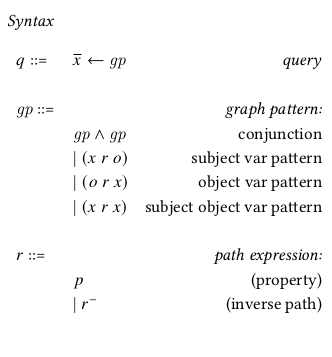
\includegraphics[scale=0.6]{pictures/leinbergSyntax}
    \caption{sintassi delle query \\ SPARQL CQ}
    \label{fig:leinbergerSyntax}
\end{figure}
\newpage
\section[Ontologie]{Ontologie}
La definizione comunemente accettata di ontologia è \textit{una specifica formale ed esplicita di una concettualizzazione condivisa} \cite{goy2015ontologies}. Un modo di rappresentarle è attraverso particolari linguaggi altamente espressivi appartenenti a una famiglia di formalismi chiamati logiche descrittive (DL). Le informazioni sul dominio di interesse vengono espresse in maniera formale tramite formule logiche di due tipologie. Una tipologia fa parte della cosiddetta T-Box e sono asserzioni sulla terminologia, componendo uno schema. L'altra fa parte della A-Box ed è usata per fare asserzioni su individui (astratti), quindi modella le istanze significative. Il T-Box contiene formule logiche (assiomi) che mettono in relazione delle \textit{concept expressions} per modellare il dominio di riferimento, ad esempio il fatto che  uno Student è una Persona. Una \textit{base di conoscenza} è quindi l'insieme di asserzioni presenti sia nel T-Box che nell'A-Box.\\
Nel contesto del Web Semantico, la raccomandazione W3C \textit{Web Ontology Language (OWL)} è una famiglia di linguaggi ontologici altamente espressivi basati sul linguaggio descrittivo $\mathcal{SROIQ}$ \cite{baader2017introductionDL}. Quello che andremo a mostrare noi nella sezione dei costrutti sintattici DL è il più semplice sottoinsieme $\mathcal{ALCOIQ}$.
Grazie alla forma logica delle informazioni, è possibile definire un ragionamento automatico\footnote{\ i.e. tramite un algoritmo deterministico, cioè eseguibile da un computer} che permette di svolgere operazioni di inferenza sugli individui concreti, ad esempio inferire che il nodo \textit{x} di un grafo RDF è uno Studente, ma anche eseguire compiti più astratti, come capire se un concetto è soddisfacibile. Questi compiti sono alla base di ogni reasoner, come ad esempio HermiT \cite{HermiT}, Pellet \cite{Pellet} e Fact++ \cite{Fact++}.\\

\subsection[Logica  descrittiva $\mathcal{ALCOIQ}$]{Logica  descrittiva $\mathcal{ALCOIQ}$}
Questa introduzione e gli esempi sono presi dal libro \cite{baader2017introductionDL}, che contiene un'ottima introduzione alle logiche descrittive. Per non divagare troppo dal motivo per cui spieghiamo questi concetti, ovvero per permettere ai lettori meno esperti delle ontologie di capire la terminologia usata in questa tesi, la logica utilizzata in questa sezione sarà principalmente $\mathcal{ALCOIQ}$. Per questo motivo, useremo anche esempi e tabelle prese dall'introduzione della tesi di dottorato di Leinberger \cite{leinbergerphdthesis}. L'acronimo $\mathcal{ALCOIQ}$ descrive i costrutti sintattici disponibili nel linguaggio (\autoref{fig:SintassiCD}). I costrutti di base sono contenuti in $\mathcal{ALC}$ (\textit{Attributive Language with Complements}), e le estensioni introdotte sono spiegate nella \autoref{tab:ALCOIQExtensions}. \\\\
I linguaggi appartenenti alle logiche descrittive separano le informazioni di un argomento in una parte terminologica (\textit{T-Box}) e una di asserzioni (\textit{A-Box})\footnote{ Nelle estensioni $\mathcal{R}$ del linguaggio $\mathcal{ALC}$, come ad esempio in OWL ($\mathcal{SROIQ}$), esiste una terzo insieme di asserzioni chiamati R-Box. Dentro vengono contenute asserzioni per creare legami fra i ruoli (come equivalenza o sotto-ruolo). Per saperne di più consultare \cite{baader2017introductionDL}}. In altre parole, il T-Box definisce informazioni sulla correlazioni dei concetti (e.g. Studente è una Persona che frequenta un corso), simile a uno schema di un database. L’A-Box descrive invece la rappresentazione concreta dei concetti (e.g. Alice è una Persona), molto più simile alle istanze di una tabella relazionale. La combinazione di entrambe viene definita una \textit{Knowledge Base} (KB).
Nelle logiche descrittive si assume di voler descrivere un’astrazione della realtà d’interesse, e che questa sia popolata da elementi. Per descrivere quest'ultimi utilizziamo tre componenti:
\begin{description}
	\item[Concept expression] Anche chiamato concept description, è un insieme di elementi e può essere visto come un predicato unario. Le concept expressions sono definite a partire dai \textit{nomi di concetti} e dai \textit{nomi di ruolo}. Sono definiti induttivamente dall’insieme di tutte le regole sintattiche del linguaggio considerato (vedi \autoref{fig:SintassiCD}). L’insieme che una concept description rappresenta è chiamato la sua \textit{estensione}. Per esempio, Persona è un concetto, e Alice è un elemento (nell’estensione) di Persona.
	\item[Role expression] relazione binaria sugli elementi. È definito atomicamente da un \textit{nome}. L'unico altro costrutto in $\mathcal{ALCOIQ}$ è il ruolo inverso, che non è nient'altro che la coppia di entità in ordine inverso. Se un ruolo \textit{r} mette in relazione un elemento con un altro, si definisce quest’ultimo un \textit{r}-filler del primo (es. Alice \textit{insegna} C, C è un \textit{insegna}-filler di Alice).
	\item[Linguaggio concettuale] il linguaggio formale al centro di uno specifica logica descrittiva. Permette di costruire concept expressions e role descriptions partendo da nomi di concetti, nomi di ruoli e altre primitive.
\end{description}

Di solito un linguaggio DL permette di costruire concetti utilizzando gli operatori comuni alla logica del prim’ordine (e.g. $\sqcap, \sqcup, \exists, \forall \text{ e } \neg)$, ma ci possono essere varie estensioni che possono essere considerate per un linguaggio. L'estensione che può risultare più strana nella \autoref{fig:SintassiCD} è la regola (Restrizione num. richiesto), che richiede che permette di esprimere il vincolo di avere almeno \textit{n} \textit{r}-filler della concept expression C. Per fare un esempio servirebbe definire l'ambito in cui vengono utilizzate le concept e le role expression, che è proprio quello che introdurremo nella sezione successiva.\\
\begin{figure}[b!]
	\begin{center}	
		\begin{minipage}{0.6\textwidth}
			\setlength{\grammarindent}{3em} % increase separation between LHS/RHS 
			\begin{grammar}
				\let\syntleft\relax
				\let\syntright\relax
				<$\mathbf{C}$> ::= $c$ \hfill (Concetto atomico)
				\alt $\{o\}$ \hfill (Concetto nominale)
				\alt $\top$ \hfill (Top)
				\alt $\bot$ \hfill (Bottom)
				\alt $\neg \mathbf{C} $ \hfill (Negazione)
				\alt $\mathbf{C} \sqcap \mathbf{C}$ \hfill (Congiunzione)
				\alt $\mathbf{C} \sqcup \mathbf{C}$ \hfill (Disgiunzione)
				\alt $\exists\ \mathbf{R}. \mathbf{C}$ \hfill (Esistenziale)
				\alt $\forall\ \mathbf{R}. \mathbf{C}$ \hfill (Universale)
				\alt $\ge n\ \mathbf{R} . \mathbf{C}$ \hfill (Restrizione num. richiesto)
				
				<$\mathbf{R}$> ::= $r$ \hfill (Ruolo atomico)
				\alt $\mathbf{R}^-$ \hfill (Ruolo inverso)
			\end{grammar}
		\end{minipage}
		\caption{sintassi delle \textit{concept expressions} $\mathbf{C}$ e delle \textit{role descriptions} $\mathbf{R}$}
		\label{fig:SintassiCD}
	\end{center}
\end{figure}

\begin{table}
	\centering
	\begin{tabular}{c l c}
		\hline
		Estensione & Descrizione & Costrutto \\
		\hline
		$\mathcal{O}$ & Concetti nominali & $\{o\}$\\
		$\mathcal{I}$ & Ruoli inversi & $ \mathbf{R} ^-$\\
		$\mathcal{Q}$ & Restrizione del numero richiesto & $\ge n\ \mathbf{R} . \mathbf{C} $\\
		
		\hline
	\end{tabular}
	\caption{estensioni dei costrutti sintattici nel DL $\mathcal{ALCOIQ}$}
	\label{tab:ALCOIQExtensions}
\end{table}
In questa introduzione vedremo in particolare il linguaggio concettuale su cui si basa una semplificazione di OWL per permettere ai lettori meno esperti di comprendere il codice presente nel \autoref{chap:Implementazione}.
\noindent
Vedremo a breve il significato della semantica di questi costrutti, ma vale la pena di spendere qualche parola su come andranno a essere utilizzati alcuni di essi. In particolare, esistono diversi costrutti per andare a specificare degli insiemi per tutti quegli elementi che sono in relazione con un certo ruolo a un concetto particolare (parliamo di $\exists r. \mathbf{C}$,  $\forall r. \mathbf{C}$ e $\ge n\ \mathbf{R} . \mathbf{C}$). Questo ci permetterà principalmente nel T-Box di dichiarare qualche genere di concetto che deve essere in relazione con qualcosa. Ad esempio, un Celibe è un uomo che non ha consorte, ed è proprio la mancanza a caratterizzare gli elementi nell'estensione di Celibe. Questo si potrebbe andare a caratterizzare con la concept expression $\text{Uomo}\sqcap \neg\ \exists\ \textit{spostatoCon}. \text{Consorte}$.\\
Una cosa da notare è che la regola (Esistenziale) potrebbe essere espressa attraverso la (Restrizione num. richiesto). Infatti, $\exists r. \mathbf{C}$ è intuitivamente equivalente al caso particolare $\ge 1\ \mathbf{R}. \mathbf{C}$. Per un elenco di regole derivate consultare la sezione 2.2.3 di \cite{leinbergerphdthesis}.


\subsubsection*{Semantica DL}
La semantica nelle logiche descrittive è intesa attraverso un'interpretazione $\mathcal{I}$, definita come segue.
\begin{definition}
	Un'interpretazione $\mathcal{I}$ è una struttura del tipo $\mathcal{I} = (\triangle^\mathcal{I}, \cdot^\mathcal{I})$, dove $\triangle^\mathcal{I}$ è un insieme non vuoto chiamato \textit{dominio d’interpretazione} e $\cdot^\mathcal{I}$ è la \textit{funzione di interpretazione} che mappa ogni costrutto alla sua semantica definita nella \autoref{tab:SintaxSemanticsALCOIQ}.
\end{definition}
\noindent
Come è possibile intuire dalla \autoref{tab:SintaxSemanticsALCOIQ}, ai costrutti della logica descrittiva (concetti e ruoli) vengono assegnati dei significati insiemistici.
\begin{table}[t!]
	\centering
	\footnotesize
	\begin{tabular}{ l l l }
		\hline
		\textbf{Costrutto} & \textbf{Sintassi} & \textbf{Semantica}\\ 
		\hline\\
		Concetto atomico & $c$ & $c^\mathcal{I} \subseteq \triangle^\mathcal{I}$\\
		Concetto nominale & $\{o\}$ & $\{o^\mathcal{I}\}$\\
		
		Top & $\top$ & $\triangle^\mathcal{I}$ \\
		Bottom & $\bot$ & $\emptyset$ \\
		Negazione & $\neg C$ & $\triangle^\mathcal{I} \setminus C^\mathcal{I} $\\
		Congiunzione & $C \sqcap D $ & $C^\mathcal{I} \cap D^\mathcal{I}$\\
		Disgiunzione & $C \sqcup D $ & $C^\mathcal{I} \cup D^\mathcal{I}$\\
		Esistenziale & $\exists r . C$ & $\{\ d \in \triangle^\mathcal{I}\ |\ \text{esiste}\ e \in \triangle^\mathcal{I}\ \text{t.c.}\ (d, e) \in r^\mathcal{I}\ \text{ed }\ e \in C^\mathcal{I}\ \}$\\
		Universale & $\forall r. C$  & $\{\ d \in \triangle^\mathcal{I}\ |\ \text{per ogni}\ e \in \triangle^\mathcal{I}\ \text{, allora}\ (d, e) \in r^\mathcal{I}\ \text{ed }\ e \in C^\mathcal{I}\ \}$\\
		Restrizione num. richiesto & $\ge n\ r . C$ & $\{\ o\ |\ \lvert\{ o'\ |\ (o, o') \in r^\mathcal{I}\ \text{ e } o^\mathcal{I} \in C^\mathcal{I} \}\rvert\ \ge n\ \}$ \\
		\hline \\
		Ruolo atomico & $r$ & $ r^\mathcal{I} \subseteq \triangle^\mathcal{I} \times \triangle^\mathcal{I}$\\ 
		Ruolo inverso & $r^-$ & $ \{\ (o, o') \mid\ (o', o) \in r^\mathcal{I}\ \}$
		\\
		\hline
	\end{tabular}
	\captionsetup{justification={centerlast}}
	\caption{sintassi e semantica delle concept expressions \textit{C}, \textit{D}  e del ruolo \textit{r} nella logica descrittiva $\mathcal{ALCOIQ}$ }
	\label{tab:SintaxSemanticsALCOIQ}
\end{table}
\subsubsection*{Knowledge Base $\mathcal{ALCOIQ}$}
Informalmente, possiamo dire che una Knowledge Base $\mathcal{ALC}$ è composta da 2 componenti: T-Box e A-Box. Iniziamo a definire sintassi e semantica delle T-Box.
\begin{definition}
	Dati $C$ e $D$ concept expressions, una General Concept Inclusion (GCI) è un espressione della forma $C \sqsubseteq D$. Un'insieme finito di GCI è detto T-Box. È possibile definire anche $C \equiv D$ come abbreviazione di $C \sqsubseteq D$ e $D \sqsubseteq C$.\\
	Un'interpretazione $\mathcal{I}$ \textit{soddisfa} $C \sqsubseteq D$ (scritto $\mathcal{I} \models C \sqsubseteq D $) se $C^\mathcal{I} \subseteq D^\mathcal{I}$. Un'interpretazione che soddisfa ogni GCI presente in una T-Box $\mathcal{T}$ è chiamata modello di $\mathcal{T}$ (scritto $\mathcal{I} \models \mathcal{T}$).
\end{definition}
\noindent
Una \textit{T-Box} è quindi una rappresentazione della struttura terminologica di un’ontologia. Una \textit{T-Box} contiene tutte le \textit{condizioni necessarie e sufficienti} per un elemento di far parte dell'estensione di un concetto. In questo modo esprime una gerarchia fra concept expressions. Facciamo un esempio per chiarire
\begin{align}
	\tag{$\mathcal{T}_1$.1} \label{eq:T1.1}
	\mathcal{T}_1 = \{&Person \sqsubseteq \exists\ \textit{hasName}.\top,\\
	\tag{$\mathcal{T}_1$.2} \label{eq:T1.2}
	&Student \sqsubseteq \textit{Person}\ \sqcap \ge 1\ attends.Course\ \}
\end{align}
$\mathcal{T}_1$ è una T-Box semplice, ma basterà per mostrare i casi in cui un'interpretazione non è un suo modello. Ad esempio, con riferimento a \eqref{eq:T1.1}, possiamo affermare che se qualche elemento nell'\textit{estensione} di Person non è in relazione \textit{hasName} con un qualsiasi elemento nel dominio dell'interpretazione, allora quell'interpretazione sicuramente non sarà modello per $\mathcal{T}_1$. Andiamo a vedere ora l'interpretazione $\mathcal{I}_1$, che è una degli infiniti possibili \textit{modelli} di $\mathcal{T}_1$.
\begin{align}
	\tag{$\mathcal{I}_1$} \label{eq:I1}
	\triangle^{\mathcal{I}_1} &= \{\ alice,\ bob,\ c1\ ,\ Roberto,\ bar,\ \textit{foo}\}\\
	\tag{$\mathcal{I}_1$.1} \label{eq:I1.1}
	Person^{\mathcal{I}_1} &= \{\ alice,\ bob\ \}\\
	\tag{$\mathcal{I}_1$.2} \label{eq:I1.2}
	Student^{\mathcal{I}_1} &= \{\ bob\ \} \\
	\tag{$\mathcal{I}_1$.3} \label{eq:I1.3}
	Course^{\mathcal{I}_1} &= \{\ c1,\ alice\ \}\\
	\tag{$\mathcal{I}_1$.4} \label{eq:I1.4}
	attends^{\mathcal{I}_1} &= \{\ (bob, c1)\ \}\\
	\tag{$\mathcal{I}_1$.5} \label{eq:I1.5}
	\textit{hasName}^{\mathcal{I}_1} &= \{\ (alice,\ alice),\ (alice,\ Roberto),\ (bob,\ \textit{foo})\ \}
\end{align}
Ci sono vari particolari da notare in questa interpretazione. Partendo dal dominio d'intepretazione definito in \eqref{eq:I1}, si può notare che l'elemento \textit{bar} non compare in nessuna estensione di un concetto definito da $\mathcal{T}_1$. Questo è assolutamente consentito, e dovrebbe far realizzare che non è possibile conoscere la cardinalità di $\triangle^{\mathcal{I}_1}$. Gli unici elementi che possiamo prevedere far parte del dominio sono quelli che si definiscono nell'A-Box. A differenza di \textit{bar}, \textit{foo} e \textit{Roberto} non compaiono in nessuna estensione, però sono rispettivamente \textit{hasName}-filler di \textit{bob} e \textit{alice} \eqref{eq:I1.5}. La definizione di Person in \eqref{eq:T1.1} richiede che un elemento nella sua estensione abbia almeno un \textit{hasName}-filler del concetto $\top$. Essendo \textit{foo} e \textit{Roberto} nell'estensione di $\top$ (cioè $\triangle^\mathcal{I}$), allora questo è perfettamente legale. Inoltre, sempre riguardo alla definizione \eqref{eq:T1.1}, possiamo notare come:
\begin{enumerate}[(i)]
	\item l'elemento \textit{alice} ha due \textit{hasName}-filler,
	\item uno di questi è se stesso.
\end{enumerate}
La regola (Esistenziale) ha come semantica che deve esistere un elemento \textit{r}-filler che appartiene alla (estensione della) concept expressions specificata (\autoref{tab:SintaxSemanticsALCOIQ}), (i) non crea alcun problema. Inoltre, dato che \textit{alice} è nell'estensione della concept expression $\top$, allora anche (ii) è consentito.\\
L'ultimo particolare su cui si può ragionare è il fatto che \textit{alice} sia contemporaneamente nell'estensione di Course e Person. Effettivamente è contraddittorio che una persona possa essere anche un corso. Questo caso può essere considerato un errore di modellazione del dominio, ma non è un errore dell'interpretazione bensì del T-Box $\mathcal{T}_1$. In effetti non c'è alcuna GCI che vieti ad un elemento di essere contemporaneamente in entrambe le estensioni. Quindi logicamente l'interpretazione sta solo assegnando gli elementi seguendo le regole definite dalla T-Box. Se volessimo evitare questo problema potremmo ridefinire l'asserzione \eqref{eq:T1.1} come:
\[ Person \sqsubseteq \exists\ \textit{hasName}.\top \sqcap \neg Course \]
\\
In generale, una T-Box $\mathcal{T}$ permettono di distinguere le interpretazioni che sono o non sono modelli per $\mathcal{T}$, limitando la nostra attenzione a quelle interpretazioni che modellano la porzione di realtà che si vuole modellare. Più GCI sono presenti in $\mathcal{T}$, meno modelli ha. Per la definizione formale di questa proprietà, consultare \cite{baader2017introductionDL}.
Andiamo ora a definire sintassi e semantica dell'A-Box.
\begin{definition}
	\label{def:ABox}
	Siano $\mathbf{I}$ un insieme di nomi d'individui, disgiunto dai nomi di concetti e quelli di ruolo. Per $a, b \in \mathbf{I}$, C una concept expression e $r$ un nome di ruolo, un'espressione della forma
	\begin{itemize}
		\item $a : C$ è detta un'asserzione concettuale, e
		\item $(a, b) : r$ è detta un'asserzione di ruolo.
	\end{itemize}
	Un insieme finito di asserzioni concettuali e di ruolo è detto A-Box.\\
	Una funzione d'interpretazione $\cdot^\mathcal{I}$ deve mappare ogni nome d'inviduo $a \in \mathbf{I}$ ad un elemento $a^\mathcal{I} \in \triangle^\mathcal{I}$. Un'interpretazione $\mathcal{I}$ soddisfa (scritto $\mathcal{I} \models$):
	\begin{itemize}
		\item $a : C$ se $a^\mathcal{I} \in C^\mathcal{I}$, e
		\item $(a, b) : r$ se $(a^\mathcal{I}, b^\mathcal{I}) \in r^\mathcal{I}$.
	\end{itemize}
	Un'interpretazione che soddisfa ogni asserzione concettuale e asserzione di ruolo in una A-Box $\mathcal{A}$ è detta modello di $\mathcal{A}$ ($\mathcal{I} \models \mathcal{A}$).
\end{definition}
\noindent
Si noti che negli assiomi A-Box, \textit{a} e \textit{b} non sono individui concreti, ed è necessario che sia un’interpretazione a stabilire l'elemento corrispondente da assegnare all'individuo "concettuale". Negli assiomi stiamo solo asserendo che valga una relazione del genere, ma non è detto che sia così o che due individui siano diversi. Facciamo un'esempio concreto:
\begin{align}
	\tag{$\mathcal{A}_1$.1} \label{eq:A1.1}
	\mathcal{A}_1 = \{&\textit{Alice} : \text{Person} \sqcap \text{Student},\\
	\tag{$\mathcal{A}_1$.2} \label{eq:A1.2}
	&\textit{CS600} : \text{Course},\\
	\tag{$\mathcal{A}_1$.3} \label{eq:A1.3}
	&\textit{Ph561} : \text{Course}, \\
	\tag{$\mathcal{A}_1$.4} \label{eq:A1.4}	
	&\textit{Bob} : \text{Student}\\
	\tag{$\mathcal{A}_1$.5} \label{eq:A1.5}
	&(\textit{Bob}, \textit{CS600}) : attends\\
\end{align}
\noindent
Questo A-Box ha due particolarità, riguardanti la definizione dell'individuo \textit{Alice}:
\begin{enumerate}[(i)]
	\item È definito come un'individuo del concetto $\text{Person} \sqcap \text{Student}$
	\item anche se è definito come Student, non è stato esplicitato alcun corso che frequenta, al contrario di \textit{Bob}.
\end{enumerate}
In effetti la concept expression presente nella asserzione concettuale \eqref{eq:A1.1} è ridondante, perchè Student è un sottoinsieme (semanticamente parlando) di Person. Non ha senso definirlo così, ma è comunque un'asserzione concettuale lecita. Concentriamoci invece su (ii): dato che abbiamo specificato \textit{Alice} come Student, vuol dire che deve frequentare almeno un corso, ma non abbiamo detto quale, ovvero non c'è nessuna asserzione di ruolo per della forma $(\textit{Alice}, \_) : attends$. Per la semantica definita nella \autoref{def:ABox}, però, la definizione di \textit{informazioni incomplete} non è assolutamente un problema: sarà compito dell'interpretazione, per essere un modello di $\mathcal{A}_1$, di specificare un qualsiasi elemento che faccia parte dell'estensione di Course. Ad esempio, è proposta una possibile interpretazione $\mathcal{I}_2$ (estesa dalla precedente $\mathcal{I}_1$) per cui $\models_{\mathcal{I}_2} \mathcal{A}_2$:
\begin{align}
	\tag{$\mathcal{I}_2$} \label{eq:I2}
	\triangle^{\mathcal{I}_2} &= \{\ alice,\ bob,\ c1\ ,\ Roberto,\ bar,\ \textit{foo}\}\\
	\tag{$\mathcal{I}_2$.1} \label{eq:I2.1}
	Alice^{\mathcal{I}_2} &= Bob^{\mathcal{I}_2} = bob\\
	\tag{$\mathcal{I}_2$.2} \label{eq:I2.2}
	\textit{CS600}^{\mathcal{I}_2} &= \textit{Ph561}^{\mathcal{I}_2} = c1\\
	\tag{$\mathcal{I}_2$.3} \label{eq:I2.3}
	Person^{\mathcal{I}_2} &= \{\ alice,\ bob\ \}\\
	\tag{$\mathcal{I}_2$.4} \label{eq:I2.4}
	Student^{\mathcal{I}_2} &= \{\ bob, alice\ \} \\
	\tag{$\mathcal{I}_2$.5} \label{eq:I2.5}
	Course^{\mathcal{I}_2} &= \{\ c1, \textit{alice}\ \}\\
	\tag{$\mathcal{I}_2$.6} \label{eq:I2.6}
	attends^{\mathcal{I}_2} &= \{\ (bob, c1), (alice, c1)\ \}\\
	\tag{$\mathcal{I}_2$.7} \label{eq:I2.7}
	\textit{hasName}^{\mathcal{I}_2} &= \{\ (alice,\ alice),\ (alice,\ Roberto),\ (bob,\ \textit{foo})\ \}
\end{align}
Il problema (ii) in questa interpretazione è stato risolto assegnando gli individui \textit{Alice} e \textit{Bob} allo stesso elemento, ovvero \textit{bob}. In effetti, così \textit{Alice} è a tutti gli effetti nell'estensione di Student, soddisfacendo l'asserzione concettuale. In questa interpretazione, anche l'elemento \textit{alice} è nell'estensione Student, ma i due eventi non sono correlati. Volevamo aggiungere un piccolo gioco mentale. Semplicemente, \textit{alice} adesso è nell'estensione di Student perchè la funzione d'interpretazione di $\mathcal{I}_2$ ha mappato ad \textit{attends} un'insieme in cui è presente anche una coppia in cui compare \textit{alice} come primo elemento.
\\
Ora che abbiamo definito entrambi le componenti di una Knowledge Base, possiamo procedere a darne la definizione
\begin{definition}
	Una Knowledge Base $\mathcal{KB}$ è definita dalla coppia $(\mathcal{T}, \mathcal{A})$, dove $\mathcal{T}$ è un T-Box e $\mathcal{A}$ è un A-Box. Un’interpretazione $\mathcal{I}$ è un modello di $\mathcal{KB}$ ($\mathcal{I} \models \mathcal{KB}$) se contemporaneamente $\mathcal{I} \models \mathcal{T}$ e $\mathcal{I} \models \mathcal{A}$.
\end{definition}
\noindent
In altre parole, un modello di una knowledge base è un'interpretazione che soddisfa contemporaneamente tutte le sue asserzioni, terminologiche e sugli individui.  $\mathcal{I}_2$ ad esempio è un modello della knowledge base $(\mathcal{T}_1, \mathcal{A}_1)$, mentre  $\mathcal{I}_1$ non lo è.
\subsection[Problemi di reasoning]{Problemi di reasoning}
Finora, abbiamo definito le componenti di una knowledge base DL e che cosa significhi per un'interpretazione essere un modello di essa. Di seguito illustreremo le definizioni di alcuni problemi di ragionamento che saranno necessari per capire di cosa si sta parlando principalmente nel \autoref{chap:Implementazione}. In particolare questi problemi sono alla base di ogni reasoner, strumenti in grado di eseguire attività di ragionamento. Tipicamente, nel Web Semantico, questi tool vengono basati su RDFS o OWL.
\begin{definition}
	Sia $\mathcal{A} = (\mathcal{T}, \mathcal{A})$ una knowledge base $\mathcal{ALC}$, C e D concept expressions e b un nome d'individuo. Diciamo che:
	\begin{enumerate}[(i)]
		\item C è soddisfacibile rispetto a $\mathcal{T}$, scritto $\mathcal{T} \models C$, se esiste un modello $\mathcal{I}$ di $\mathcal{T}$ e qualche $d \in \triangle^\mathcal{I}$ tale che $d \in C^\mathcal{I}$.
		\item C è sussunto da D rispetto a $\mathcal{T}$, scritto $\mathcal{T} \models C \sqsubseteq D$, se $C^\mathcal{I} = D^\mathcal{I}$ per ogni modello $\mathcal{I}$ di $\mathcal{T}$.
		\item C e D sono equivalenti rispetto a $\mathcal{T}$, scritto $\mathcal{T} \models C \equiv D$, se $C^\mathcal{I} \subseteq D^\mathcal{I}$ per ogni modello $\mathcal{I}$ di $\mathcal{T}$.
		\item $\mathcal{K}$ è consistente se esiste un modello per $\mathcal{K}$
		\item b è un'istanza di C con rispetto a $\mathcal{K}$, scritto $\mathcal{K} \models b : C$ se $b^\mathcal{I} \in C^\mathcal{I}$ per ogni modello $\mathcal{I}$ di $\mathcal{K}$
	\end{enumerate}
\end{definition}
\noindent
Tutte questi problemi possono essere ridotti alla verifica della \textit{consistenza} di una base di dati (Teorema 2.17 \cite{baader2017introductionDL}). Questo significa che è possibile usare un algoritmo per la consistenza per decidere tutti i problemi precedenti. Si noti, tuttavia, che ci sono altri problemi di ragionamento non menzionati la cui riduzione non è possibile, ed anche se lo fosse la complessità del problema sarebbe intrattabile. Uno di questi è decidere le risposte esatte di una conjunctive query, per cui nel linguaggio $\mathcal{SROIQ}$ (proprio quello di OWL) la sua decidibilità è una questione ancora non risolta, mentre per lo stesso linguaggio la verifica della consistenza è decidibile e \textsc{N2ExpTime} completo \cite{baader2017introductionDL}. Non andremo ad approfondire nel dettaglio la complessità, per i lettori interessati su questa questione consigliamo di approfondire il Capitolo 5 e 7 di \cite{baader2017introductionDL}.


\clearemptydoublepage
\chapter[Stato dell'arte]{Stato dell'arte}
Per poter considerare l'utilizzo dei tipi per il Web Semantico, è necessario analizzare lo stato dell'arte in cui si ritrova questo ambito di ricerca.
Questo capitolo si presta utile per apprendere il vocabolario utilizzato durante tutta la tesi, nonché fornire approfondimenti su nozioni che potrebbero essere date per scontate.
Verranno riassunte le basi dei linguaggi funzionali, così come le componenti del Web Semantico.
\section[Linguaggi funzionali]{Linguaggi funzionali}
\section[Web Semantico]{Web Semantico}
Il World Wide Web è ormai una gigantesca e consolidata rete di conoscenza, che però nasconde un difetto fondamentale per l'utilizzo di queste informazioni da parte di un agente artificiale. Infatti il linguaggio di rappresentazione, HTML, è stato pensato per la fruizione umana dei suoi contenuti piuttosto che di una macchina. Ciò rende difficile per quest'ultime capire il significato delle informazioni presenti nel web. Uno degli obiettivi del Web Semantico, presentato per la prima volta nel 2001 in \cite{berners2001semantic}, è cambiare questo paradigma human-centered, permettendo agli agenti artificiali di interpretare e processare la conoscenza presente senza alcun tipo di aiuto umano. È necessario descrivere le informazioni attraverso metadati espressivi, strutturandoli arbitrariamente, che ne spieghino la semantica in un modo che una macchina possa comprenderla.

Nel corso degli anni, nella letteratura sono state presentate diverse soluzioni: dagli albori di questo ambito, in cui i dati erano rappresentati in maniera strutturata e formale dalle ontologie, si è giunti alla rappresentazione superficiale ma efficiente del paradigma dei Linked (Open) Data. Questa sezione vuole introdurre agli standard di rappresentazione e recupero dei dati citati in questo lavoro.

\subsection[Resource Description Framework]{Resource Description Framework}
Il Resource Description Framework\footnote{https://www.w3.org/RDF/} (RDF d'ora in poi) è una specifica W3C (World Wide Web Consortium) che fornisce un modello per descrivere risorse nel Web attraverso delle annotazioni. Un termine (o \emph{tripla}) RDF è della forma:
\[ < \text{soggetto},\ \text{proprietà},\ \text{oggetto} > \]
Un'insieme di triple, chiamato un grafo RDF, permettono di descrivere un grafo diretto etichettato dove le risorse descritte sono i nodi e le proprietà sono gli archi.
\begin{figure}[h]
  \begin{minipage}{0.3\linewidth}
    \centering
    \begin{tikzpicture}[
        node distance = 15mm and 15mm,
        V/.style = {rounded corners, draw, fill=gray!30},
        every edge quotes/.style = {auto, font=\footnotesize, sloped}
      ]
      \begin{scope}[nodes=V]
        \node (1)   {Pizza};
        \node (2) [right=of 1]    {Margherita};
        \node (3) [below =of 2]    {Mozzarella};
        \node (4) [left=of 3]    {Vegetarian};
      \end{scope}
      \draw[->, ultra thick]   (2)  edge["isA"] (1)
      (2)  edge["madeOf"] (3)
      (4)  edge["canEat"] (2);
    \end{tikzpicture}
  \end{minipage}
  \hspace{5mm}
  \begin{minipage}{0.7\linewidth}
    \begin{alignat*}{4}
      G_1 = \{ (\  & \text{Margherita},\  &  & isA,      &  & \text{Pizza}        &  & ),  \\
      (\           & \text{Margherita},\  &  & madeOf,\  &  & \text{Mozzarella}\  &  & ),  \\
      (\           & \text{Vegetarian},\  &  & canEat,\  &  & \text{Mozzarella}\  &  & )\}
    \end{alignat*}
  \end{minipage}
  \caption{Esempio di un grafo RDF $G_1$ (sx.) e sotto forma di insieme di triple (dx.)}
\end{figure}

Invece di chiamare un nodo semplicemente \singlenodegraph{Margherita}. I valori di queste classi (in letteratura \emph{letterali}) possono essere riferimenti tramite URI a risorse Web, oppure
\clearemptydoublepage
\chapter[Implementazione]{Implementazione}
\label{chap:Implementazione}
Il software si pone l'obiettivo di verificare se una query e l'utilizzo del suo risultato sia corretto o meno. Per le query si tratta di verificare se sia abitata o meno. Il nostro software è formato da due componenti: un modulo Reasoner, scritto in java che si occupa di determinare l'abitabilità delle query, e un modulo scritto in OCaml che si occupa di determinare la correttezza di un programma scritto su file testuale.

\section{OCaml Module - Le query}
\label{sec:OCaml Module - Le query}
L'idea alla base del modulo OCaml è la seguente:
\begin{enumerate}
    \item l'utente inserisce la query di cui testare l'abitabilità in un file di testo.
    \item la query viene parsata in un tipo Query
    \item sul tipo Query vengono inferiti gli assiomi di Leinberger
    \item viene invocato il -Reasoner e gli vengono passati gli assiomi appena inferiti.
    \item il risultato viene mostrato all'utente
\end{enumerate}

Per generare il parser, ho utilizzato il programma OCamlyacc, un compilatore di compilatori, ispirandomi alla grammatica delle query descritta da Leinberger\ref{fig:leinbergerSyntax}. 

Per definire i token che compongono la grammatica invece mi sono avvalso di OCamllex, un generatore di lexer.


Dunque, come funziona il Parser? Esso riconosce la grammatica e genera un tipo Query\ref{fig:querType}, che racchiude tutte le informazioni presenti all'interno della query in formato testuale. 

\begin{figure}[H]
    \centering
    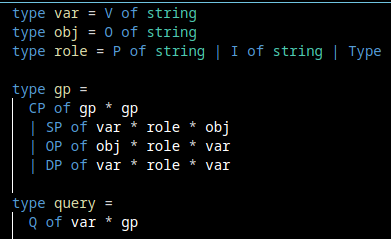
\includegraphics[scale=0.7]{pictures/queryType.png}
    \caption{tipo Query corrispondente alla sintassi delle query SPARQL CQ}
    \label{fig:querType}
\end{figure}


Per esempio, scrivendo questa query sul file di input:

\[ query \ x \ <- \ (x \ type \ Pizza \ AND \ x \ hasTopping \ y \ AND \ y \ type \ GorgonzolaTopping) \]

otteniamo il seguente tipo Query così costruito: 

\[ Q \  (V \ x, \\
    CP(SP(V \ x,\ TYPE, \ ,\ CP)\]

Introduciamo il tipo ClassExpression, definito ispirandosi alle regole di derivazione degli assiomi di Leiberger.
\begin{figure}[H]
    \centering
    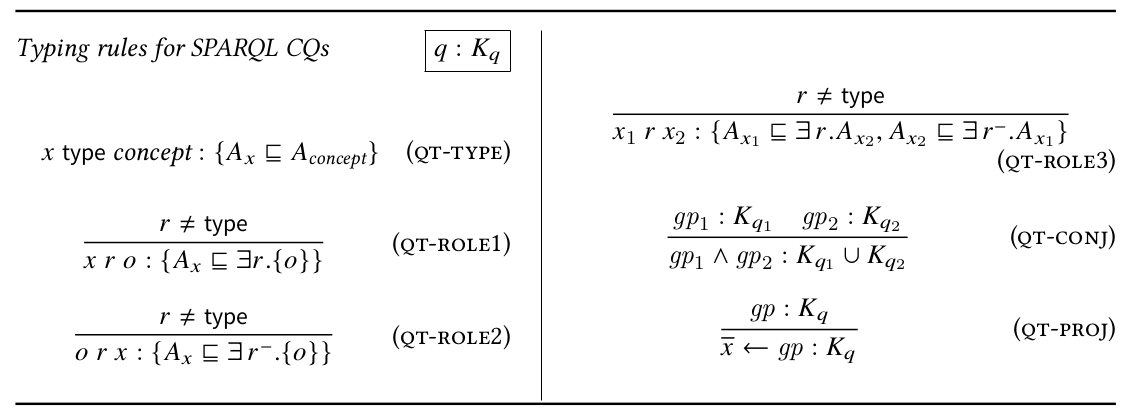
\includegraphics[width=\textwidth]{pictures/leinbergAxiom.png}
    \caption{Regole di derivazione degli assiomi di Leiberger}
    \label{fig:leinbergerAxiom}
\end{figure}

\begin{figure}[H]
    \centering
    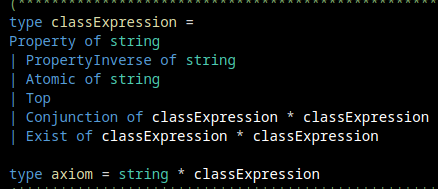
\includegraphics[width=\textwidth]{pictures/classExpressionType.png}
    \caption{Il tipo ClassExpression e Axiom}
    \label{fig:enter-label}
\end{figure}
Successivamente, il tipo Query viene convertito in una lista di Axiom dalla funzione axiomiserQuery, che implementa le regole di derivazione di Leinberger [\ref{fig:leinbergerAxiom}]\\ \\L'esempio diventa dunque:
\[ (x, Pizza) :: (x, Exist(Property(hasTopping),Atomic(y))) :: \]\[ (y, Exists(PropertyInverse(hasTopping), Atomic(x))) ::
      (y, GorgonzolaTopping) :: []
 \]
        
Infine, la lista di assiomi viene convertita in stringa secondo la sintassi \(A_{x} : C\), ove C è la traduzione in sintassi di Manchestern della classExpression corrispondente. 
\\\\ L'esempio diventa dunque
\[ x : Pizza : x : hasTopping \ SOME \ y : y : INVERSE \ hasTopping x : y : GorgonzolaTopping\]
Viene dunque invocato il modulo Reasoner e gli viene passato come parametro la lista in formato stringa. La risposta, true o false, viene poi mostrata a video all'utente. 

\newpage   
\section{Reasoner}
Il modulo Reasoner utilizza due risorse:
\begin{enumerate}
    \item Il file HermiT.jar\cite{HermiT}, che implementa il reasoner sviluppato dall'università di Oxford, capace di eseguire ragionamenti sulle ontologie.
    \item Il file DLQueryExample\cite{DLQueryExample} utilizzato per parsare una stringa in una ClassExpression, che è utilizzabile HermiT.
\end{enumerate}

Ma come funziona il modulo? Esso prende in input, in formato stringa, una lista di assiomi di Leinberger, ognuno forma \(A_{x} : C\), con semantica \( A_{x}\sqsubseteq C \).
\\\(A_{x}\) è un concetto atomico. "C" è una concept expression scritta nella "Manchester OWL syntax" \cite{ManchesterOWLSyntax}, e viene trasformato dal DLQueryParser in un oggetto ClassExpression. L'idea iniziale era di creare noi un parser che trasformasse una stringa in un oggetto ClassExpression, poi ci siamo imbattuti nella Manchester OWL syntax che presentava già un parsificatore capace di realizzare esattamente quello che volevamo. Allora ho adattato il tutto affinché lavorasse su questa particolare sintassi.

Utilizzando poi la OWLDataFactory (factory delle OWLApi che permette la costruzione di OWLAxiom e di dichiarare OWLClass) e HermiT\cite{HermiT}, dichiariamo all'interno dell'ontologia tutti i concetti atomici che compaiono negli assiomi di Leinberger\ref{fig:leinbergerSyntax}, corrispondenti alle variabili della query.

\begin{figure}[H]
    \centering
    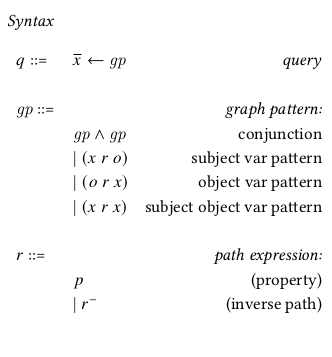
\includegraphics[scale=0.6]{pictures/leinbergSyntax}
    \caption{sintassi delle query \\ SPARQL CQ}
    \label{fig:leinbergerSyntax}
\end{figure}

Successivamente per ogni assioma creiamo un OWLSubClassOfAxiom, in cui viene specificata la relazione di sottoclasse tra il concetto atomico(le variabili) e la sua ClassExpression corrispondente(concept expression).

Infine chiediamo al reasoner HermiT di testare la soddisfacibilità di ogni concetto atomico presente negli assiomi di Leinberger. Se sono tutti soddisfacibili, allora significa che la query è abitabile, altrimenti non lo è.
    
    \newpage
    \section{Il linguaggio $\boldsymbol{\lambda_{DL}}$}
    Quando si effettua una computazione basata su ontologie, il processo di ragionamento è portato avanti a run time, e se si scoprono assiomi non soddisfacibili 
    il programma potrebbe essere soggetto a errori. Non è quindi possibile garantire che un'esecuzione termini correttamente, ovvero si otterrà il risultato aspettato. 
    Il nostro obiettivo è quello riuscire a catturare questi errori prima dell'esecuzione, andando ad assicurare una computazione senza errori run-time che dipendono dalla base di conoscenza. 
    Vorremmo quindi valutare vantaggi e efficienza di un controllo statico, sfruttando i sistemi di tipi per assicurare la correttezza statica del programma, rispetto a 
    un'ontologia basata sulle logiche descrittive (in particolare OWL). Sforzi verso questa direzioni sono stati già proposti nella tesi di dottorato di Martin Leinberger, 
    in cui propone un lambda calcolo tipato esteso con interrogazioni SPARQL a basi di triple RDF e costrutti della logica descrittiva come tipi chiamato $\lambda_{DL}$.
    \\ Il linguaggio garantisce di eseguire delle QUERY SPARQL che rispettano A-Box e T-Box dell'ontologia, spostando il controllo dell'abitabilità durante il type checking e
    permettendo di tipare i nodi ritornati dalle Query tramite le concept expressions della logica descrittiva.
    L'esempio successivo, preso dalla tesi di Leinberger, mostra un programma scritto in $\lambda_{DL}$ che espone chiaramente le potenzialità del linguaggio.
    \begin{figure}[h]
        \captionsetup{singlelinecheck = false}
        $K_4 = $\{Students $\sqsubseteq$ Person
        \\Professor $\sqsubseteq$ Person\}
        \begin{minted}[escapeinside=||,mathescape=true, autogobble]{ocaml}
            (head (query x |$\leftarrow$| x type Student)).x
        \end{minted}
        \caption{Programma in $\lambda_{DL}$ avente come knowledge base $K_4$}
    \end{figure}
    \\Il programma esegue una query SPARQL che ritorna una lista di mapping tra la variabile \textbf{x} e nodi del grafo RDF che rispettino il vincolo
    \textbf{x type Students}. Successivamente prendiamo il primo elemento della lista (\textbf{head}) e lo proiettiamo sulla variabile \textbf{x} (\textbf{(...).x}).
    Il sistema di tipo ci permette di:
    \begin{itemize}
        \item stabilire la correttezza della query, costruendo degli assiomi dalla sua struttura e richiamando un reasoner.
        \item dare un tipo ai nodi ritornati dalla query. Nel nostro esempio tutta l'espressione è di tipo \textbf{Students} e grazie al subtyping e al fatto
            che nella knowledge base sappiamo che Students $\sqsubseteq$ Person è anche ti tipo \textbf{Person}.
    \end{itemize}
    L'implementazione si concentra solo sul type system, i riferimenti agli aspetti più teorici del linguaggio insieme alla sintassi e le regole di valutazione
    si possono trovare nella tesi di Leiberger.
    Vale la pena per\`o accennare che il linguaggio è corretto, ovvero un termine chiuso e ben tipato non si blocca durante la valutazione.
    La corretteza è dimostrata da Leinberger attraverso due teoremi:
    \begin{theorem}
        (Progress in $\lambda_{DL}$): sia t un termine ben tipato e chiuso. se t non è un valore, allora esiste una termine t' tale che
        t $\xrightarrow[]{\text{K}}$ t'. Se $\Gamma$, K $\vdash$ t : T, allora t è un valore o un termine contenente head nil[T] e tail nil[T] oppure esiste
        un t' per cui t $\xrightarrow[]{\text{K}}$ t'
    \end{theorem}
    \begin{theorem}
        (Preservation in $\lambda_{DL}$): Sia t un termine e T un tipo. Se un tipo è assegnato a t, scritto $\Gamma,K \vdash t : T$ e t $\xrightarrow[]{\text{K}}$ t'
        allora, $\Gamma,K \vdash t' : T$
    \end{theorem}
    Entrambe le dimostrazioni sono per induzione su $\Gamma,K \vdash t : T$ e i dettagli si possono trovare nella tesi di Leinberger.
\newpage
\section{Type Checking} \label{sec:Type Checking}
        Per implementare il type checking abbiamo usato come base il lambda calcolo tipato proposto dal libro di \textbf{Benjamin C. Pierce "Types and Programming Languages"}.
        Nella tesi parleremo strettamente delle regole di tipo e della loro implementazione per quanto riguarda la valutazioni si veda il libro di Pierce e la tesi di Leinberger.
        Il linguaggio presenta le principali caratteristiche di un \textbf{ $\boldsymbol{\lambda}$-calcolo tipato} con l'aggiunta dei \textbf{Record}, le \textbf{Liste} e le \textbf{Query SPARQL}.
        \begin{figure}[h] 
            \begin{minted}{ocaml}
                type Term =
                      TmVar of info * int * int 
                    | TmTrue of info 
                    | TmFalse of info 
                    | TmIf of info * term * term * term 
                    | TmRecord of info * (string * term) list 
                    | TmProj of info * term * string 
                    | TmAbs of info * string * ty * term 
                    | TmApp of info * term * term 
                    | TmLet of info * string * term * term 
                    | TmFix of info * term 
                    | TmZero of info 
                    | TmSucc of info * term 
                    | TmPred of info * term 
                    | TmIsZero of info * term 
                    | TmNil of info * ty 
                    | TmCons of info * term * term 
                    | TmIsNil of info * term 
                    | TmHead of info * term 
                    | TmTail of info * term  
                    | TmQuery of info * var * gp
                    | TmRoleProj of info * term * role
                    | TmEq of info * term * term
                    | TmNode of info * string
            \end{minted}
        \caption{termini del $\lambda_{DL}$}
        \end{figure}
        TmRecord e quello che ci permette di avere nel nostro linguaggio termini come:
        \begin{minted}{OCaml}
        {x = 4; y = 0; z = 4}
        \end{minted}
        dove $x, y, z$ sono le etichette del record, mentre $4, 0, 4$ sono i termini associati alle etichette. Nella implementazione corrispondono rispettivamente alla
        stringa e al termine della lista. TmProj invece è la proiezione di un record su una etichetta, quindi riprentendo dall'esmpio precedente 
        \begin{minted}{Ocaml}
        {x = 4; y = 0; z = 4}.x
        \end{minted}
        il record proiettato su x, come ci si aspetta, sarà valutato nel valore associato alla etichetta: 4.
        Le liste sono costruite ricorsivamente con \textbf{TmNil} e \textbf{TmCons} e sono presenti delle operazioni sulle liste espresse dai termini \textbf{TmIsNil},
        \textbf{TmHead} e \textbf{TmTail}
        \begin{figure}[h]
            \begin{minted}[escapeinside =|, autogobble]{python}
                [1, 0]        TmCons (TmSucc (TmZero)) (TmCons (TmZero) (TmNil))
                head  [1, 0]  TmHead (TmCons (TmSucc (TmZero)) (TmCons (TmZero) (TmNil)))
                tail  [1, 0]  TmTail (TmCons (TmSucc (TmZero)) (TmCons (TmZero) (TmNil)))
                isNil [1, 0]  TmIsNil (TmCons (TmSucc (TmZero)) (TmCons (TmZero) (TmNil)))
            \end{minted}
        \caption{esempi di termini con liste}
        \end{figure}
        Infine le query sono implementate come descritto nella sezione precedente.
        \\I tipi hanno un datatype apposito. Oltre ad avere i classici tipi booleani (TyBool), numeri natoruali (TyNat) e il tipo freccia (TyArr) 
        sono presenti i tipi per i nuovi costrutti (TyRecord, TyList, TyConcept). Il tipo \textbf{Top} è usato per il subtyping, in particolare per
        qualsiasi tipo $T$ vale che $\boldsymbol{T <: Top}$. La figura sottostante mostra il datatype costruito in OCaml.
        \begin{minted}{ocaml}
            type Ty =
                  TyTop 
                | TyBool 
                | TyRecord of (string * ty) list 
                | TyArr of ty * ty 
                | TyNat 
                | TyList of ty
                | TyConcept of ce
        \end{minted}
        Alcuni esempi di tipi assegnati ai relativi termini possono essere:
        \begin{minted}{ocaml}
            {x = 4; y = 0; z = 4} : {x : Nat, y : Nat, z = Nat}
            [1, 0] : List Nat
            query x <- x type students : List {x : Ax}
        \end{minted}
        dove i tipi segnati sono un versione semplificata e più leggibile per indicare il termine costruito dal datatype ty:
        \begin{minted}{ocaml}
            TyRecord([("x", TyNat); ("y", TyNat); ("z", TyNat)])
            TyList TyNat
            TyConcept Atomic("x")
        \end{minted}
        Ora che abbiamo introdotto i costruttori di tipi utilizzati possiamo paralre dell'algoritmo di typing.
        Come suggerito dal libro "Types and Programming Languages" viene utilizzata una funzione ricorsiva per determinare il tipo di un termine da un contesto
        inizialmente vuoto.
        \begin{minted}{ocaml}
            typeof : Context -> Term -> Ty
        \end{minted}
        typeof effettua pattern matching sul termine passato come argomento per decidere quale regola applicare. La maggior parte delle regole sono puramente
        sintattiche quindi typeof è sufficiente per la loro implementazione, altre come le regole di subtyping o [T-ADD] è necessario utilizzare funzioni di supporto
        oppure modificare l'implementazione delle regole precedenti. Un semplice esempio di implementazione di una regola di tipo è quello di [T-APP].
        $$\myruleN{\Gamma \vdash t_1 : T_1 \rightarrow T_2 \quad \Gamma \vdash t_2 : T_1}{\Gamma \vdash t_1 \: t_2 : T_2}{T-APP}$$
        la cui implementazione diventerà:
        \begin{minted}[escapeinside=||,mathescape=true, autogobble]{ocaml}
            let rec typeof ctx t =
                match t with
                |$\vdots $|
                TmApp(fi,t1,t2) ->
                    let tyT1 = typeof ctx t1 in
                    let tyT2 = typeof ctx t2 in
                    (match ctx tyT1 with
                        TyArr(tyT11,tyT12) ->
                          if subtype ctx tyT2 tyT11 then tyT12
                          else error fi "parameter type mismatch"
                        | _ -> error fi "arrow type expected")

                |$\vdots$|
        \end{minted}
        Prima attraverso pattern matching si controlla che il termine passato sia un'applicazione tra altri due termini $t1$ e $t2$. Successivamente
        viene effettuata la chiamata ricorsiva su $t1$ e $t2$ per ottenere i loro tipi $tyT1$ e $tyT2$ rispettivamente. Effettuando di nuovo pattern matching
        su $tyT1$ si verifica che sia un tipo freccia $tyT11 \rightarrow tyT12$. Infine se $tyT2 <: tyT11$ allora si può stabilire che $t1 \; t2$ ha tipo $tyT12$.
        Come si vede dalla implementazione di [T-APP] è stata utilizzata una funzione per verificare il subtyping, ritornando true se e solo se $Ty_1 <: Ty_2$. 
        \begin{minted}{ocaml}
            subtype : Context -> Ty -> Ty -> Bool
        \end{minted}
        Il linguaggio $\lambda_{DL}$ presenta il subtyping classico tra funzioni, record e liste le cui regole si possono trovare sia nella tesi di Leinberger che
        in "Types and Programming Languages". L'implementazione della funzione \textbf{subtype} è molto diretta rispetto alle regole. Come per \textbf{typeof}
        si procede con il pattern matching tra i tipi passati come argomento e confrontando la loro struttura si può stabilire se sono in relazione di sottotipo.
        Per esempio la regola \textbf{[S-LIST]}
        $$\myruleN{T <: T'}{List \; T <: List \; T'}{S-LIST}$$
        \\ viene implementata con con:
        \begin{minted}[escapeinside =**, mathescape=true, autogobble]{ocaml}
            let rec subtype ctx tyS tyT =
                tyeqv ctx tyS tyT ||
                match (tyS,tyT) with
                    *$\vdots$*
                     (TyList(tyS1),TyList(tyT1)) -> subtype ctx tyS1 tyT1
                    *$\vdots$*
        \end{minted}
        La funzione tyeqv controlla l'ugualianza tra due tipi siccome la relazione di subtyping è riflessiva. l'ultime due funzioni di supporto
        utilizzate per il typing calcolano il least upper bound (\textbf{join}) e il greatest lower bound (\textbf{meet}) tra due tipi.
        \begin{minted}{ocaml}
            meet : Context -> Ty -> Ty -> Ty
            join : Context -> Ty -> Ty -> Ty
        \end{minted}
        La figura sottostante mostra le regole di tipo aggiunte da Leinberger nel $\lambda_{DL}$ e nelle sottosezioni successive analizzeremo regola per regola
        il loro significato e ne mostreremo una possibile implementazione.  
        \textbf{aggiungere correttezza, obiettivo del type system e nelle introduzioni introdurre con esempi il linguaggio, aggiungere i riferimenti alla sezione precedente}
        \begin{figure}[h]
        \[\begin{array}{c}
            \myruleN{\Gamma,K \vdash t_1 : C_1 \quad K \vDash C_1 \sqsubseteq \exists r . \top}
            {\Gamma,K \vdash t_1.r : \textrm{List}(\exists r^- . C_1)}
            {T-PROJ}
            \qquad
            \myruleN{\Gamma,K \vdash : C \quad \Gamma,K \vdash t_2 : D}
            {\Gamma, K \vdash t_1 = t_2 : \textrm{Bool}}
            {T-EQ-NOM}
            \qquad
            \\\\
            \myruleN{\Gamma,K \vdash t_1 : \Pi_1 \quad \Gamma,K \vdash t_2 : \Pi_1}
            {\Gamma,K \vdash t_1 = t_2 : \textrm{Bool}}
            {T-EQ-PRIM}
            \qquad
            \myruleN{}{\Gamma,K \vdash o : \{o\}}{T-NOMINAL}
            \\\\
            \myruleN{q:K_q \quad \textrm{head}(q) = \{l_i^{i \in 1...m}\} \quad \forall x \in \textrm{Vars}(q) : K \cup K_q \nvDash A_x \sqsubseteq \bot}
            {\Gamma,K \cup K_q \vdash \textrm{query} \; q : \{l_i : A_{l_i}^{i \in 1...m}\} list}
            {T-QUERY}
            \\\\
            \myruleN{\Gamma,K \cup \{A_i \sqsubseteq C_i^{i \in 1...n}\} \vdash t : A_j^{1 \leq j \leq n} \quad K \cup \{A_i \sqsubseteq C_i^{i \in 1...n}\} \vDash A_j \sqsubseteq D^{1 \leq j \leq n}}
            {\Gamma,K \vdash t : D}
            {T-ADD}
            \\\\
            \myruleN{K \vDash C \sqsubseteq D}{K \vdash C <: D}{S-CONCEPT}
        \end{array}\]
        \caption{nuove regole di tipo per $\lambda_{DL}$}
        \end{figure}
        \subsection{La regola [T-PROJ]}
            L'implementazione della regola [T-PROJ] segue alla lettera la definizione teorica in particolare abbiamo che la condizione $\Gamma,K \vdash t_1 : C_1$
            è verificata attraverso il pattern matching (.1) in cui controlliamo che il tipo $t$ sia una concept expression \textbf{TyConcept(C)}. La seconda ipotesi
            $K \vDash C_1 \sqsubseteq \exists r . \top$ invece richiede la creazione di una nuova funzione:
            \begin{minted}[escapeinside=||,mathescape=true, framesep=4mm, autogobble]{ocaml}
                subconcept : ConceptExpression -> ConceptExpression -> Bool
            \end{minted}
            la funzione subconcept prende in input due concept expression $C_1$ e $C_2$ e ritorna $true$ se e solo se $C_1 \sqsubseteq C_2$. Quindi passando a subconcept
            \textbf{C} e \textbf{Exist(Property(s), Top)} (.2) come argomento verifichiamo la seconda condizione.
            \\Infine le conclusioni della regola $\Gamma,K \vdash t_1.r : \textrm{List}(\exists r^- . C_1)$ affermano facendo la proiezione del termine $T_1$ attraverso $r$
            otteniamo una lista di concept expression $\exists r^- . C_1$, per questo motivo la funzione typeof ritorna  \textbf{TyList(TyConcept(Exist(PropertyInverse(s), c)))} (.3).
            \begin{figure}[h] 
                \begin{minted}[escapeinside=||,mathescape=true, frame=lines, framesep=4mm, autogobble]{ocaml}
                    let rec typeof ctx t =
                        match t with
                        |$\vdots $|
                        TmRoleProj(fi, t, Property(s)) ->
                            (match typeof ctx t with
                            TyConcept(C) as t ->                                        .1
                                if subconcept C Exist(Property(s), Top) then            .2
                                    TyList(TyConcept(Exist(PropertyInverse(s), c)))     .3
                                else error fi "argument of role projection 
                                                is not a proper subconcept")
                            _ -> error fi "argument of role projection 
                                            is not a Concept Expression"
                        |$\vdots$|
                \end{minted}
            \caption{implementazione OCaml della regola [T-PROJ]}
            \end{figure}

            \subsection{La regola [T-QUERY]}
            [T-QUERY] è la regola utilizzata per derivare il tipo di una query SPARQL. Per semplicità, rispetto alla teoria, prendiamo in considerazione solo le query
            aventi una variabile, ovvero dove l'insieme $Head(q)$ contiene un solo elemento. Anche questa regola richiede di consultare un reasoner per stabilire se
            gli assiomi generati dal typing della query q siano soddisfacibili $\forall x \in \textrm{Vars}(q) : K \cup K_q \nvDash A_x \sqsubseteq \bot$.
            Nella definizione la funzione $Vars(q)$ ritorna l'insieme di tutte le variabili utilizzate nella query.
            \begin{figure}[h]
                \begin{minted}[escapeinside=||,mathescape=true, frame=lines, framesep=4mm, autogobble]{ocaml}
                    let rec typeof ctx t =
                        match t with
                        |$\vdots $|
                        TmQuery(fi, var, gp) ->
                            if allSatisfiable(axioms(gp), var) then
                            TyList(TyRecord(var, TyConcept(Atomic var))) else
                                error fi "axioms unsatisibale"
                        |$\vdots$|
                \end{minted}
            \caption{implementazione OCaml della regola [T-QUERY]}
            \end{figure}
            \\Nella implementazione, per verificare le ipotesi utilizziamo due funzioni di supporto. la prima:
            \begin{minted}{OCaml}
            axioms: Gp -> Axiom List
            \end{minted}
            ritorna la lista degli assiomi dal graph pattern della query. mentre la seconda
            \begin{minted}{OCaml}
            allSatisfiable: Axioms List -> Var -> Bool
            \end{minted}
            è la funzione che interroga la knowledge base per verificare che la lista degli assiomi sia soddisfacibile. Infine una volta verificate le ipotesi possiamo
            ritornare
            \\\textbf{TyList(TyRecord(var, TyConcept(Atomic \; var)))} che corrisponde a $\Gamma,K \cup K_q \vdash \textrm{query} \; q : \{l_i : A_{l_i}^{i \in 1...m}\} list$
            con l'unica differenza che nella nostra implementazione i record contengono una sola label, quella della unica variabile in $Head(q)$. Abbiamo deciso di
            mantenere la lista di record nonostante la nostra semplificazine sulle query per rendere un futuro aggiornamento facile da implementare.
            \subsection{La regola [T-ADD]}
            [T-ADD] è la regola la cui implementazione è più interessante. Siccome non siamo di fronte ad una regola puramente sintattica
            non è possibile fare pattern matching sul termine per capire quando applicarla.
            Prima di parlare dell'implementazione è importante capire a cosa serve e come viene utilizzada: [T-QUERY] assegna alle variabili in testa alla query
            il tipo concept expression $A_x$ quando abbiamo un assioma nella query della forma $K_q = A_x \sqsubseteq D$, ma $A_x$ non sono propriamente da usare sintatticamente nel programma.
            \\L'obiettivo è dare un significato al tipo $A_x$, in modo simile a una classica regola di subtyping. Quindi è possibile assegnate una concept espression $D$
            a un termine t solo se è possibile assegnare a t $A_x$ usando una knowledge base $\Gamma,K \cup \{A_i \sqsubseteq C_i^{i \in 1...n}\} \vdash t : A_j^{1 \leq j \leq n}$
            e se K $\cup \{A_i \sqsubseteq C_i^{i \in 1...n}\} \vDash A_j \sqsubseteq D^{1 \leq j \leq n}$.
            \\Come suggerito da Leinberger, abbiamo implementato la regola aggiungendo gli assiomi $K_q$ alla knowledge base durante la funzione \textbf{allSatisfiable}.
            così insieme alla regola \textbf{S-CONCEPT} è possibile risalire alla concept $D$ senza avere bisogno di [T-ADD].
            \subsection{La regola [S-CONCEPT]}
            Il linguaggio cotruito da Leinberger permette il subtyping tipi, quindi oltre a quello tra tipi classici è stato necessario aggiungere un modo per gestire
            anche quello tra le concept expression.
            \begin{figure}[h]
                \begin{minted}[escapeinside=||,mathescape=true, frame=lines, framesep=4mm, autogobble]{ocaml}
                    let rec subtype ctx tyS tyT =
                        tyeqv ctx tyS tyT ||
                        match (tyS,tyT) with
                        |$\vdots $|
                            (TyConcept(ceS1),TyConcept(ceT1)) -> subconcept ceS1 ceT1
                        |$\vdots$|
                \end{minted}
            \caption{implementazione OCaml della regola [S-CONCEPT]}
            \end{figure}
            Nella implementazione richiamiamo la funzione subconcept per il controllo della ipotesi $K \vDash C \sqsubseteq D$. La differenza maggiore rispetto alla teoria
            risiede nel fatto che anche in questo caso [S-CONCEPT] non è una regola sintattica. La funzione subtype ha tipo:
            \begin{minted}[]{ocaml}
                subtype : Context -> Ty -> Ty -> Bool
            \end{minted}
            Prende in input un contesto e due tipi e ritorna $true$ se e solo se $K \vDash C \sqsubseteq D$. la funzione subtype viene poi richiamata su tutte le regole
            in cui il subtyping è utilizzabile. Ad esempio nella regola [T-APP] si controlla che l'argomento passato a una astrazione sia sottotipo del tipo atteso dalla astrazione (\textbf{Controvarianza}).
            \begin{minted}[escapeinside=||,mathescape=true, frame=lines, framesep=4mm, autogobble]{ocaml}
                let rec typeof ctx t =
                    match t with
                    |$\vdots $|
                    TmApp(fi,t1,t2) ->
                    let tyT1 = typeof ctx t1 in
                    let tyT2 = typeof ctx t2 in
                    (match ctx tyT1 with
                        TyArr(tyT11,tyT12) ->
                          if subtype ctx tyT2 tyT11 then tyT12
                          else error fi "parameter type mismatch"
                        _ -> error fi "arrow type expected")
                    |$\vdots$|
            \end{minted}












        
        
\clearemptydoublepage

\chapter[Direzioni di ricerca future]{Direzioni di ricerca future}
\label{chap:FutureWork}

Nei capitoli precedenti abbiamo esplorato una parte dell'esistente lavoro relativo alla ricerca sull'uso dei sistemi di tipi statici nel contesto della 
rappresentazione della conoscenza, in particolare applicati al formalismo delle ontologie OWL \cite{OWL}. In breve, si può pensare di utilizzare i 
linguaggi con sistemi di tipi statici per realizzare modelli e strumenti per  il Web Semantico, come alternative o come supporto statico al reasoning 
dinamico basato sulle logiche descrittive (si vedano l'introduzione nel Capitolo \ref{chap:preliminaries} e una prima survey sullo stato dell'arte nel Capitolo \ref{chap:State-of-art}).

In questo capitolo, proponiamo alcune congetture di direzioni di ricerca future, ispirate da quanto abbiamo imparato dal nostro studio preliminare e dalle 
discussioni con i colleghi esperti di Web Semantico. Al momento, non abbiamo argomenti né formali né empirici per validare queste idee, tuttavia riteniamo 
che siano un punto di partenza promettente per studi successivi.

Ricordiamo che un'ontologia OWL ha due componenti: \textsc{T-Box} e \textsc{A-Box}. I costrutti nella \textsc{T-Box} sono la "componente terminologica" che descrive un dominio di 
interesse, definendone classi e proprietà, similmente a un vocabolario di quel dato dominio. I costrutti di \textsc{A-Box} sono la "componente assertiva", intesi come fatti associati al modello concettuale descritto dalla \textsc{T-Box}. I costrutti \textsc{A-Box} devono essere \textsc{T-Box}-compliant: sono asserzioni che utilizzano il 
vocabolario definito dalla \textsc{T-Box}. I costrutti \textsc{T-Box} sono talvolta associati a classi orientate agli oggetti e i costrutti \textsc{A-Box} associati a istanze di tali 
classi\footnote{Da \url{https://en.wikipedia.org/wiki/Abox}}.

Utilizzare strumenti logici come i sistemi di tipi per fare reasoning potrebbe sembrare una direzione di ricerca che va nel senso contrario 
rispetto alla preferenza corrente dell'applicazione di tecniche sub-logiche, legate soprattutto al machine learning, anche al reasoning nel web 
semantico. Tali tecniche sfruttano talvolta solo dati estratti dalle asserzioni sugli individui (ovvero dai costrutti della \textsc{A-Box}, spesso rappresentati 
come triple RDF e relativo knowledge graph), soprattutto per questioni di efficienza. In effetti, sembra che al presente  la ricerca sulle ontologie abbia 
perso momento, perché nella loro interezza (\textsc{T-Box} e \textsc{A-Box}) sono troppo formalmente complesse per fare ragionamenti totalmente automatizzati (si vedano i 
concetti preliminari nel \autoref{chap:preliminaries}). Tuttavia, ci sembra che ci siano delle potenzialità da esplorare per poter tornare a fare reasoning più 
sofisticato, senza perdere troppo in efficienza.
\\
Ci sono almeno due strade che possiamo percorrere:
\begin{enumerate}
	\item L'utilizzo di linguaggi funzionali tipati, quali Haskell\footnote{\url{www.haskell.org}} e Ocaml\footnote{\url{www.ocaml.org}} per programmare applicazioni che manipolano le ontologie, con il 
	vantaggio di usare linguaggi basati su un alto livello di astrazione, che quindi permettono uno sviluppo del software modulare, più facile da correggere e da 
	mantenere, e anche più vicino al livello simbolico che caratterizza il reasoning semantico. 
	\item Lo studio di sistemi di tipi statici che garantiscano proprietà 
	interessanti ai programmi, certificati dal sistema di tipi stesso. Il fatto di usare tipi statici, cioè controllati a tempo di compilazione (scelta ancora 
	poco adottata nel reasoning semantico, basata sull'uso di interpreti), potrebbe essere una risposta ai problemi di efficienza per certe proprietà che avrebbe 
	senso controllare a priori, e/o nel caso di grandi quantità di dati.
\end{enumerate}

L'esempio principale che abbiamo scelto di mostrare in questo lavoro, il calcolo $\lambda_{DL}$ di Martin Leinberger presentato nella sua tesi di dottorato 
"Type-safe Programming for the Semantic Web" \cite{leinbergerphdthesis} (si veda il \autoref{chap:Implementazione}) è certamente un esempio del \mbox{Punto 2}. Questo calcolo offre un sistema di tipi per decidere a tempo di compilazione se una query SPARQL è abitata, ovvero se è possibile che produca un risultato quando interpretata, oppure al 
contrario, se non abitata, sappiamo già a priori che la query non produrrà alcun risultato.  Il nostro lavoro di implementazione, però, ci ha dato qualche 
indicazione anche relativamente al Punto 1: per esempio, abbiamo scoperto che il linguaggio Ocaml ha delle librerie utili per il parsing e per interfacciarsi 
con la shell del sistema operativo, oltre ad avere un miglior sistema di error management e il vantaggio di non dover usare monadi, come invece avrebbe 
richiesto Haskell.

Concludiamo questo lavoro con una serie di proposte che potrebbero essere esplorate nel futuro, nelle direzioni menzionate sopra. Queste proposte 
nascono da alcuni proficui scambi di idee con Marco Antonio Stranisci, Rossana Damiano e Antonio Lieto del Dipartimento di Informatica dell'Università 
di Torino.

\section{Tipi per il query rewriting}
Il \textit{query rewriting} è una tecnica per mappare una query SPARQL in un'altra \cite{fQuery}, utile nelle situazioni in cui l'utente non ha una conoscenza precisa del vocabolario e 
del lessico utilizzato nell'ontologia di interesse e in cui lo studio approfondito di questa ontologia non sarebbe vantaggioso, normalmente per motivi di tempo. Un esempio semplice potrebbe essere quello di un'ontologia che descrive razze di cani-poliziotto senza avere il concetto \texttt{Cane} esplicito nel suo vocabolario.
Se l'utente utilizzasse \texttt{Cane} nelle sue query, per esempio per cercare tutti i cani con il manto di un certo colore, non otterrebbe nessun risultato. Una combinazione di strumenti per l'analisi del linguaggio naturale e un sistema di tipi che controlli la correttezza (per esempio nel senso di Leinberger \cite{leinbergerphdthesis}) della query trasformata  dopo l'analisi potrebbe essere un buon strumento per il query rewriting. Un'altra applicazione di simili tecniche potrebbe agevolare l'uso di ontologie il cui vocabolario è in una lingua straniera.

Una direzione pratica per fare esperimenti potrebbe essere utilizzare reti di parole implementate sotto forma di dizionari enciclopedici 
basati sulle ontologie come Babelnet \footnote{Si veda \url{https://babelnet.org/}} per misurare una "distanza semantica"  che intercorre fra due lemmi, per poter decidere quale si avvicina di più a quello usato dall'utente. Possiamo immaginare che si misuri la distanza semantica che intercorre fra la parola della query e le parole nel vocabolario dell'ontologia. Quella con la distanza minore sarà la parola riscritta all'interno della query. Ci potrebbero essere ambiguità, intesa come due o più parole semanticamente alla stessa distanza da quella presente nella query. Per ognuna di queste parole semanticamente simili, si genererebbe dunque una query.
Per controllare l'abitabilità delle query riscritte, sapendo che ogni query ha uno e un solo insieme di assiomi alla Leinberger (si veda \autoref{chap:Implementazione}), si potrebbe generare un tipo che è un insieme di assiomi alla Leinberger se la riscrittura è senza ambiguità, oppure un insieme di insiemi di questi assiomi se la query è effettivamente ambigua.

Questa direzione di ricerca potrebbe beneficiare dallo studio degli approcci per la generazione di query SPARQL partendo da query in linguaggio naturale (questi approcci vengono definiti \textit{Text2SPARQL}). Anche se la quantità di letteratura su questi approcci è ancora scarsa, i lavori \cite{Hu2021NaturalLQ, Evseev2020SPARQLQG} e il tool OSCAR \cite{OSCAR} possono fornire un'idea della struttura dei modelli utilizzati.

\section{Tipi per costruire e ristrutturare ontologie}
Nei processi di creazione di un'ontologia, la tendenza attuale è di sfruttare il più possibile risorse esistenti, sfruttando conoscenze organizzate in 
Terminology Services \cite{ledl2016describing,vandenbussche2017linked} o utilizzando \emph{search engine appositi} come 
Swoogle \cite{swoogle} o Watson \cite{watson} per trovare ontologie. I risultati della ricerca vengono poi sottoposti a processi di valutazione 
(\emph{assesment}), comparazione (\emph{comparison}) e integrazione (\emph{integration}) per ottenere i migliori risultati rispetto al dominio d'interesse. Tali attività possono però essere soggette a errori, poiché le ambiguità, le incoerenze e l'eterogeneità delle ontologie esistenti 
possono influire sui risultati rispetto a diversi punti di vista. Si possono avere, infatti, eterogeneità sintattica, terminologica, concettuale e semiotica \cite{carriero2020OntoReuse}. Questo processo di costruzione di un'ontologia è quindi dispendioso a livello di tempo perché richiede un'accurata verifica da parte degli esperti di ontologie, di cui non è possibile rimuovere il contributo dal processo creativo. L'obiettivo di questa direzione di ricerca sarebbe fornire allo sviluppatore degli strumenti formali da utilizzare durante il processo di creazione/evoluzione di un'ontologia, per aiutarlo nel capire se il suo processo stia effettivamente producendo il risultato desiderato (per esempio offrendo una nozione precisa di equivalenza tra ontologie) e/o suggerire cambiamenti o entità da riutilizzare o aggiungere, sfruttando proprietà come la composizionalità (ovvero la proprietà che garantisce la correttezza della composizione delle parti di un artefatto sviluppate separatamente, posto che le parti obbediscano a certe condizioni), tipica dei linguaggi tipati staticamente. Vista la tendenza attuale di sviluppare un'ontologia partendo da risorse ontologiche esistenti, la proprietà di composizionalità applicata alle ontologie potrebbe automatizzare parte dei compiti di ristrutturazione delle risorse ontologiche da riutilizzare, come la modularizzazione, per considerare solo la parte rilevante per il processo in atto. Un punto di partenza promettente è la metodologia NeOn \cite{NeOn}, che offre una serie di scenari che sono di supporto ai processi di creazione e evoluzione delle ontologie. Uno di questi scenari propone una lista di criteri comparativi per valutare la bontà delle soluzioni possibili (si veda il \autoref{chap:State-of-art}).

Per questa direzione di ricerca servirebbe un caso di studio che potrebbe beneficiare di tali strumenti formali, utili nel caso in cui si voglia progettare 
da zero una nuova ontologia o nel caso di "major changes" di ontologie già esistenti. Al presente sono disponibili ontologie molto generali, ben stabilizzate 
e facilmente adattabili ai casi particolari, per cui può sembrare che questa direzione sia poco promettente, ma riteniamo che sia comunque meritevole di 
esplorazioni future.

\section{\large Usi innovativi di strumenti esistenti: tipi per l'XML}
Il linguaggio funzionale tipato chiamato $\mathbb{C}$Duce\footnote{\url{www.cduce.org}} \cite{CDuce}, orientato alla manipolazione dell'XML \cite{XML}, permette di produrre XML corretto a partire da specifiche formali (tipi) e di scrivere query corrette per le basi di dati espresse in XML. Siccome RDF/XML è uno degli standard W3C per la 
rappresentazione di ontologie OWL, si potrebbe pensare di adattare $\mathbb{C}$Duce per la generazione di ontologie a partire da specifiche astratte e query corrette su 
di esse, come strumento possibilmente alternativo o di supporto a Protègè \cite{protege}. Nel seguito diamo un'intuizione di come $\mathbb{C}$Duce potrebbe essere usato per rappresentare costrutti ontologici.

Per quanto riguarda la formalizzazione della \textsc{T-Box}, $\mathbb{C}$Duce permette di distinguere le varie parti della struttura di un tag, in questo modo siamo in grado di 
estrarre tutte le parti necessarie per distinguere un tag di descrizione da uno, per esempio, che descrive la meta-relazione di sottoclasse. In questo modo, 
siccome le classi e sottoclassi sono simili a quelle dei linguaggi di programmazione, possiamo generare dal documento la struttura gerarchica e le classi 
coinvolte. Segue un frammento di codice $\mathbb{C}$Duce che mostra quanto detto sopra:
\begin{minted}{xml}
	<rdfs:Class rdf:about="Man">
	<rdfs:subClassOf rdf:resource="Person"/>
	</rdfs:Class>
\end{minted}
Altro esempio riguardo alle relazioni tra dati è il seguente:
\begin{minted}{xml}
	<rdf:Property rdf:about="hasWife">
	<rdfs:domain rdf:resource="Man"/>
	<rdfs:range rdf:resource="Woman"/>
	</rdf:Property>
\end{minted}

Questo esempio è più interessante perché specifica il dominio e codominio della proprietà. In $\mathbb{C}$Duce è possibile estrarre i valori dei campi di un tag e 
quindi andare a prendere i valori \code{Man} e \code{Woman}, e di conseguenza ritrovare i tipi associati a queste stringhe. Perciò è possibile definire un costruttore 
di tipo \code{hasWife}, definito come \code{Man  Woman  hasWife}, su cui successivamente si può fare pattern matching per ricavare dominio e codominio, oltre a 
eventualmente definire la relazione inversa. 

Come esempio di asserzione di una \textsc{A-Box}, prendiamo il seguente frammento di codice:
\begin{minted}{xml}
	<rdf:Description rdf:about="James">
	<rdf:type rdf:resource="Man"/>
	</rdf:Description>
\end{minted}
L'unico caso sensato con cui si può definire questo tag è tramite l'instanziazione di un valore \code{James} che sia di tipo \code{Man}. 
Ampliando gli esempi precedenti con i tag delle ontologie e RDF si potrebbe ricostruire il "Tipo" di un'ontologia, semplificando così le operazioni di 
modifica sia in profondità che in  ampiezza. $\mathbb{C}$Duce permette anche di fare il procedimento opposto, cioè di passare da un suo tipo ad uno schema XML, 
permettendo di riportare l'ontologia, modificata precedentemente tramite il suo tipo, nel formato RDF/XML.

Un'altra applicazione possibile di $\mathbb{C}$Duce riguarda il merging di ontologie (espresse in XML), ossia il processo in cui singoli concetti, assiomi e affermazioni di ontologie sorgenti vengono fusi insieme in un nuovo modello. L'idea è ridurre il problema del merging di ontologie al merging di tipi. Prese due ontologie da fondere, le si trasforma tramite $\mathbb{C}$Duce in tipi, si esegue il merging tra di essi e poi il tipo risultante lo si 
utilizza per generare l'ontologia finale.

\section{\large Tipi per lo schema concettuale Functional Requirements for Bibliographic Records (FRBR)}
Per Functional Requirements for Bibliographic Records (FRBR) \cite{frbr} si intende uno schema concettuale sviluppato dalla International Federation of Library 
Associations and Institutions (IFLA), realizzato tramite modello entità-relazione allo scopo di dare una rappresentazione semi-formale alle informazioni 
bibliografiche\footnote{Da https://it.wikipedia.org/wiki/Functional_Requirements_for_Bibliographic_Records}. FRBR è nato per descrivere tre gruppi di informazioni:

\begin{itemize}
	\item le opere
	\item le organizzazioni o persone che sono responsabili delle opere
	\item i soggetti delle opere (es. i luoghi o concetti espressi da un libro)
\end{itemize}
\noindent
Al presente l'uso maggiore che se ne sta facendo è rispetto al Punto 1. Le opere sono classificate secondo i livelli:
\paragraph{Livelli astratti}
	\begin{itemize}
		\item \textit{work} (opera)
		\item \textit{expression} (espressione)
	\end{itemize}
\paragraph{Livelli fisici}
	\begin{itemize}
		\item \textit{manifestation} (manifestazione)
		\item \textit{item} (oggetto concreto)
	\end{itemize}
\noindent
FRBR specifica anche delle particolare relazione fra livelli di entità:
\begin{itemize}
	\item un work \textit{è realizzato attraverso} una o più expression;
	\item una expression \textit{si materializza in} una o più manifestation;
	\item una manifestation \textit{è rappresentata da} uno o più item.
\end{itemize}
\noindent
È da tenere presente che questa non è una gerarchia di livelli, ovvero nessun livello di entità è inteso concettualmente come un sotto-concetto di un'altro. 
Questa descrizione è più simile al concetto di composizione dei linguaggi object-oriented (o dei modelli entity-relationship), in cui ogni livello inferiore 
della specifica FRBR è in relazione con quello superiore tramite una relazione di composizione (part-of).

FRBR descrive relazioni fra le opere, chiamate \textit{content relationships}. Possono essere suddivise in 3 gruppi:
\begin{itemize}
	\item \textsc{Equivalent} - Facsimile, Copy
	\item \textsc{Derivative} - Translation, Revision
	\item \textsc{Descriptive} - Review, Annotated Edition
\end{itemize}
Queste relazioni fra opere sono poi ereditate anche dalle sottostanti espressioni, manifestazioni e item in maniera transitiva.
\\
Un esempio di rappresentazione FRBR è la seguente, relativa all'opera "The Last of Us"\footnote{\url{https://www.playstation.com/en-us/the-last-of-us/} <3}:
\begin{description}
	\item[Work:] The Last of Us Part I (VideoGame), The Last of Us (Serie TV).
	\item[Expression:] The Last of Us Part I traduzione italiana e versione orginale.
	\item[Manifestation:]:  The Last Of Us versione Disco e versione digitale.
	\item[Item:]: Copia fisica (o digitale) di The Last of Us.
\end{description}
\noindent
Un primo passo verso una formalizzazione di questa rappresentazione semi-formale delle informazioni bibliografiche è proprio il tentativo di mapparla su 
concetti tipici dei linguaggi di programmazione e di modellazione dei dati, sui quali è poi più facile definire dei sistemi di tipi. Ma a che servirebbero i 
tipi in questo contesto? Abbiamo individuato alcuni possibili ambiti e casi di studio:

\begin{description}
	\item[Retrieving di duplicati di un’opera:] Un semplice esempio per spiegare l'intuizione di questo caso è il problema di avere due record per lo stesso libro, uno con il titolo scritto con iniziale maiuscola e l'altro con l'iniziale minuscola. Il livello \emph{work} è il più astratto e quindi potrebbe essere visto come un tipo: per usare un termine object-oriented è una sorta di classe astratta senza attributi. Potrebbe essere 
	interessante arricchire un \emph{work} con degli attributi, legati fra loro con assiomi legati al dominio, e regole per inferire relazioni come la similarità 
	tra \emph{work} da applicare alle istanze dei livelli inferiori, in particolare agli \emph{item}. Tipi di questo genere potrebbero essere usati per la gestione dei 
	duplicati: controllare che ci siano dei duplicati si ridurrebbe nel cercare un cluster di \emph{item} astratti/descritti dallo stesso \emph{work} preso in 
	considerazione. La prima fase consisterebbe nell'uso di uno strumento di estrazione del tipo degli \emph{item} (il \emph{work}). Successivamente verrebbe applicata 
	un'operazione di match tra i tipi, che astraggono le proprietà basilari degli \emph{item}, semplificando e quindi rendendo meno oneroso l'operazione di match. 
	Una variante potrebbe essere quella di non avere un sistema di tipi \emph{work} di partenza, ma di crearli quando si incontra un \emph{item} che non ha ancora un \emph{work} 
	con cui etichettarlo. Se poi inferendo un tipo di un \emph{item} si risale ad un tipo \emph{work} già precedentemente costruito questo si aggiungerebbe a tale tipo \emph{work}. Il sistema potrebbe avere anche tipi più complessi, 
	ad esempio esprimenti connettivi logici quali \textsc{OR} e \textsc{AND}, qualora ci fossero delle ambiguità di assegnamento di certi item a più tipi \emph{work}.
	\item[Ristrutturazione di biblioteche virtuali:] si potrebbe pensare di utilizzare i tipi \emph{work} (definiti seguendo l'idea di cui sopra) per convertire 
	dati non strutturati (o strutturati secondo formati diversi) nel formato FRBR: un'idea potrebbe essere il costruire un tipo prototipo, che sia a 
	livello \emph{work} (o più in alto eventualmente, tramite il metalivello \emph{family of works}, che si dovrebbe esplorare più a fondo) che permetta di andare a 
	costruire un cluster di quelle tassonomie che descrivono lo stesso \emph{work} (o magari \emph{work} equivalenti, secondo le content relationships menzionate sopra). 
	Per i libri catalogati normalmente, la maggior parte dei casi sarebbe probabilmente un controllo sintattico sulle proprietà espresse dagli attributi di 
	catalogozione, ma questo ambito diventa più interessante se si parla di manoscritti o \emph{item} parzialmente distrutti di cui non si hanno informazioni 
	complete (addirittura potrebbe mancare il titolo, oltre a altri attributi di catalogazione).
\end{description}
Per entrambi gli ambiti ci sono molte domande aperte, tra cui:
\begin{enumerate}
	\item Quali tipi sono necessari? È sufficiente considerare \emph{work} (o \emph{family of work}) o bisogna costruire i tipi anche per gli strati sottostanti? Occorre 
	approfondire lo studio di FRBR e interrogare gli esperti, bibliotecari e scienziati della conoscenza, rispetto alle loro esigenze.
	\item Qualsiasi siano le proprietà che si vogliono garantire tramite uno o più sistemi di tipi è comunque richiesta parte di analisi sintattica o anche 
	forme di analisi del linguaggio naturale? Quasi sicuramente sì, così come sarebbero necessari esperti del dominio per generare dei tipi/assiomi 
	sufficientemente informativi che andranno a popolare la knowledge base FRBR.
	\item Al momento stiamo considerando gli \emph{item} come termini e i \emph{work} come tipi, non considerando i livelli intermedi. Potrebbe anche essere una 
	semplificazione utile per cominciare, ma ci poniamo come ulteriore punto di riflessione il considerare come tipo che dà proprietà agli \emph{item} una 
	combinazione dei primi tre livelli.
\end{enumerate}
\noindent
Una strada parallela potrebbe essere quella di estendere FRBR, andando ad aggiungere ulteriori livelli per l'astrazione del livello \emph{work} e, di conseguenza, 
avere a disposizione tipi più espressivi. Un'ulteriore strato potrebbe essere quello dei concetti originali, o archetipi, da cui prende ispirazione o introduce l'opera. Un archetipo rappresenta l'idea platonica di un concetto, che poi viene integrata o ereditata dai \emph{work}. Questo potrebbe essere utile 
per i ricercatori che indagano sull'eredità dei concetti espressi in opere antiche, per verificare quali opere derivano da altre e via dicendo.

\section{Tipi per la riproducibilità nell'Open Science}
Le idee alla base della riproducibilità sono: 
\begin{enumerate}[I)]
	\item un esperimento scientifico deve poter essere riprodotto; 
	\item la ricerca deve avvenire in modo aperto e corale. 
\end{enumerate}
Un forma di tipaggio simile al tagging potrebbe essere per esempio usata come meta-dati sui dati degli esperimenti, da utilizzare, per esempio, per 
fare inferenze utili a tracciarne la provenienza. Questa tipologia di controllo sembra essere adatto da essere eseguito staticamente.
\clearemptydoublepage

%%%% TAIL OF THE DOCUMENT
\backmatter
%list of figures
\listoffigures
\clearemptydoublepage
%list of tables
\listoftables
\clearemptydoublepage
%bibliography
\bibliographystyle{acm}
\bibliography{bibliography/bibThesis}
\addcontentsline{toc}{chapter}{Bibliography}
\clearemptydoublepage


\end{document}
